
%***************************************************************************
%
% CreditCruncher - A portfolio credit risk valorator
% Copyright (C) 2003-2010 Gerard Torrent
%
% This program is free software; you can redistribute it and/or
% modify it under the terms of the GNU General Public License
% as published by the Free Software Foundation; either version 2
% of the License.
%
% This program is distributed in the hope that it will be useful,
% but WITHOUT ANY WARRANTY; without even the implied warranty of
% MERCHANTABILITY or FITNESS FOR A PARTICULAR PURPOSE.  See the
% GNU General Public License for more details.
%
% You should have received a copy of the GNU General Public License
% along with this program; if not, write to the Free Software
% Foundation, Inc., 59 Temple Place - Suite 330, Boston, MA 02111-1307, USA.
%
%***************************************************************************

\documentclass[a4paper,12pt,final]{article}
\usepackage{times}
\usepackage{latexsym}
\usepackage{amssymb}
\usepackage{abstract}
\usepackage[dvips]{graphicx}
\usepackage[american]{babel}
\usepackage[final]{listings}
\usepackage{fancyhdr}
\usepackage[flushmargin]{footmisc}
\usepackage{placeins}
\usepackage{verbatim}

%-----------------------------------------------------
% defining some useful values
%-----------------------------------------------------
\def\numversion{1.7}
\def\svnversion{R644}

%-----------------------------------------------------
% some format directives
%-----------------------------------------------------
\sloppy
\pagestyle{fancy}
\setlength{\parindent}{0ex}

%-----------------------------------------------------
% finally, the doc begins here
%-----------------------------------------------------
\begin{document}

\title{CCruncher - Technical Document}
\author{Gerard Torrent Gironella\\\\Version \numversion\ -\ \svnversion}
\date{\today}
\maketitle


%===========================================================================
\begin{abstract}
CCruncher computes the credit risk of massive loan portfolios 
taking into account default correlations between economic sectors. This is done 
by determining the probability distribution of portfolio loss using the Monte 
Carlo method. The simulation of borrower's default times is achieved
using a copula that combines the survival functions with the observed
sectorial correlations. Risk is obtained using the usual risk statistics, 
including Expected Loss, Value at Risk and Expected Shortfall.
\newline
\newline
\textbf{Keywords}: credit risk, Monte Carlo, survival functions, Gaussian copula, 
t-Student copula, value at risk, expected shortfall, block matrix.
\end{abstract}
\newpage


%===========================================================================
\tableofcontents
\newpage


%===========================================================================
\section{Introduction}

This introduction was originally published in \emph{Ercim News 78} \cite{ccruncher:ercim78}
as a contribution to the special theme \emph{Mathematics for Finance and Economy}.
There have been done some minor changes in order to adapt to the current situation.
\newline

Financial institutions need tools to simulate their credit portfolios in the same 
way that they simulate their equity portfolios. CCruncher allows each payment
in a massive loan portfolio to be simulated, taking into account the probability 
of default for each creditor and the correlations between them.
\newline

While the portfolios of loans given to SMEs and portfolios of corporate bonds do 
not have the glamour of the equity or foreign exchange markets, they are nevertheless 
the core business of many financial institutions. Such portfolios tend to have values 
of thousands of millions of dollars and may be composed of tens of thousands of small 
loans.
\newline

At first glance, credit portfolios may seem harmless because payments are based on 
pre-agreed dates. Nothing could be farther from the truth. Defaults frequently occur 
in clusters, affecting entire sectors of industry. The correlation between defaults 
is the main difficulty in risk assessment, and this is the rationale behind many of 
the approaches to credit risk valuation. The impact of the correlation on the loss 
distribution function is notorious, and causes an asymmetrical distribution function 
with long tails.
\newline

CCruncher is an open-source project for the simulation of massive portfolios of 
loans where the unique risk is the default risk. It is addressed to financial institutions 
searching for a well-documented and efficient tool. It consists of an engine that runs 
in batch mode and is designed to be integrated into the risk management systems of 
financial institutions for risk assessment and stress testing. The method used to 
determine the distribution of losses in the portfolio is the Monte Carlo algorithm, 
because it allows us to consider the majority of variables involved, such as the 
date and amount of each payment. This approach is conceptually equivalent to the 
valuation of portfolios of equities and derivatives using the Monte Carlo method. 
In the case of market risk, the price of the underlying assets is simulated using 
a geometric Brownian motion with a given volatility and trend. In the credit risk 
case, borrowers' defaults are simulated using a copula with given survival rates 
and correlations.
\newline

Sklar's theorem states that any multivariate distribution can be decomposed into 
two parts, the marginal distributions and a copula that reflects the structure of 
dependencies between components. This result is important because it allows us to 
separate the default probabilities from the default correlations.
\newline

CCruncher implements two of the most commonly used copulas in finance, the Normal 
and T-Student copulas. Because the default time of each borrower is modelled as a 
random variable, the size of the copula can be over 50.000, where each component 
represents a borrower. Simulating low-dimensional copulas poses no problem, but many 
of the algorithms operating in low dimensions are unsuitable for large dimensions. 
To solve this problem, the Cholesky decomposition was adapted to operate with a large 
correlation matrix composed of blocks, in order to reduce the memory space and the 
number of operations involved.

\begin{figure}[!hbt]
\begin{center}
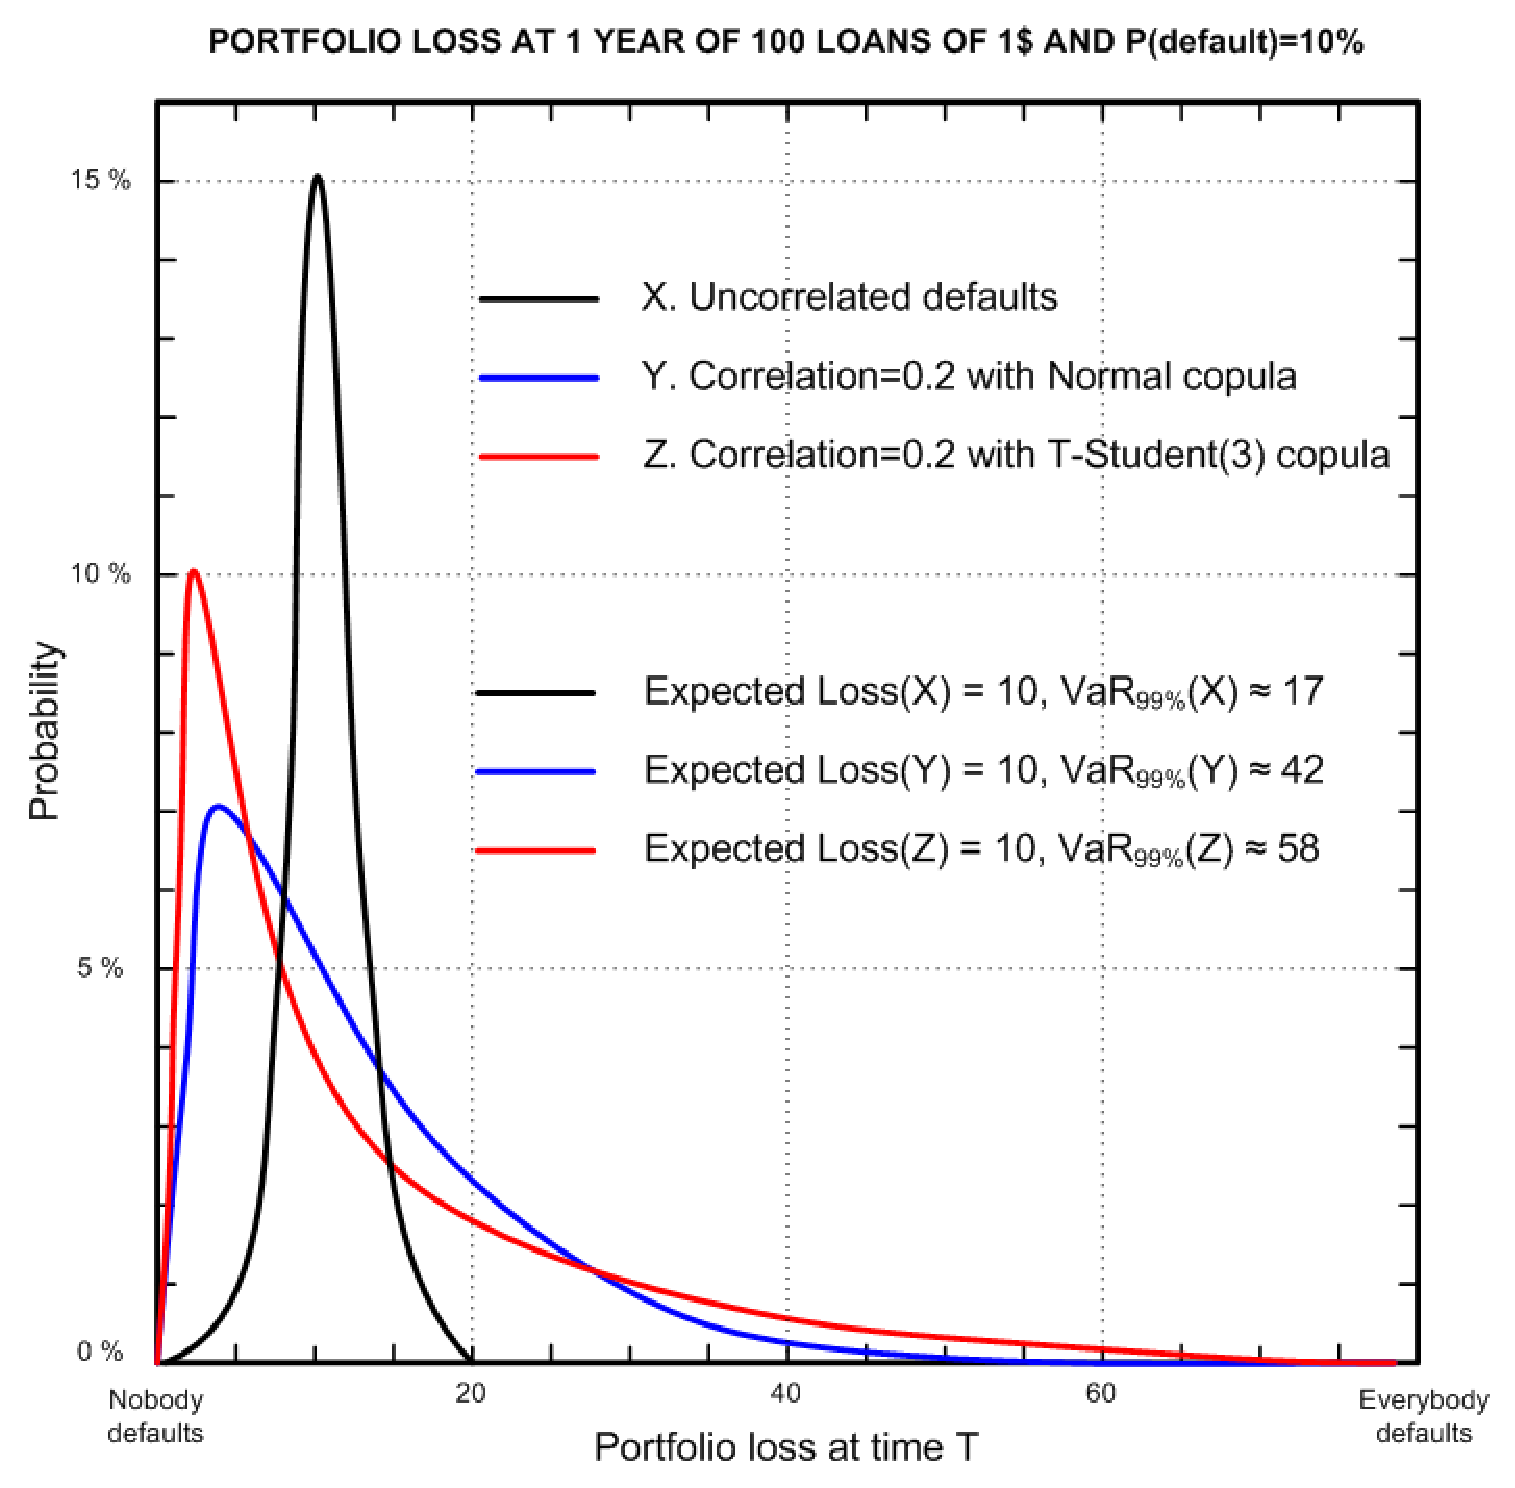
\includegraphics[height=10cm]{./images/ercim78.eps}
\caption{Impact of correlation and copula selection on portfolio loss distribution}
\label{survival}
\end{center}
\end{figure}
\FloatBarrier

Each Monte Carlo run simulates the default time for each debtor by combining a copula 
sampling with the survival functions. This default time is used to determine the loss 
caused by the default, mitigated by an estimated recovery at a given time. The default 
amount is discounted to the present value using the interest rate provided by the yield 
curve. The sum of all losses provides the loss value of the portfolio for that simulation. 
The completion of thousands of simulations allows us to obtain the loss distribution 
function and compute the usual risk indicators, such as the Value at Risk or Expected 
Shortfall. Depending on the portfolio size and the required accuracy, the computational 
cost may be high.
\newline

CCruncher is currently a one-man project with no financial support, and is looking 
for collaborators with expertise in applied and/or theoretical financial mathematics 
to participate in a GPL (GNU General Public License) structure. The CCruncher 
system has been tested against both simple hand-made portfolios and large automatically 
generated portfolios. Future work is being considered to add stochastic recovery rates, 
and stochastic exposures, and the creation of a graphical interface to 
make the tool available to the public, such as portfolio bond managers.

\begin{comment}
\subsection{Credit Risk Models}
TODO: merton models, actuarial models, econometric models, intensity models, copula models
TODO: Comparison with other methods (CreditRisk+, CreditMetrics)
\end{comment}

%===========================================================================
\section{Parameters}

This section explains the input parameters that are required by CCruncher.

%---------------------------------------------------------------------------
\subsection{Ratings and Survival Functions}
A credit rating estimates the probability that an individual or corporation 
will pay back a loan. A poor rating indicates a high risk of defaulting.
Each rating has an associated survival function. This function indicates 
the probability that a borrower with an initial rating ($X$) will not have 
defaulted at time $t$. 

\begin{figure}[!hbt]
\begin{center}
\includegraphics[height=10cm, angle=-90]{./images/survival.ps}
\caption{Survival functions}
\label{survival}
\end{center}
\end{figure}
\FloatBarrier

The survival data is often not available, and where it is available, it is 
often inconsistent or not representative. For this reason, it is better to work 
with the transition matrix, assuming that the rating transitions follow a Markov 
model. Appendix \ref{ap:tmatrix} shows how to determine the survival functions 
using the transition matrix.

%---------------------------------------------------------------------------
\subsection{Sectors and Correlations}
\label{sectors}
The risk of a credit portfolio depends crucially on correlations between 
economic sectors. These sectors are groupings of companies that react similarly to 
economic conditions. Some examples of sectors include: energy, financial, technology, 
media and entertainment, utilities, and health care. Default correlations between 
sectors measure the default time dependence between the defined sectors. This 
can be expressed in tabular form:

\begin{center}
\begin{displaymath}
\begin{array}{cc}
\begin{array}{c|ccc}
                    & \mathrm{Sector}_1 & \dots  & \mathrm{Sector}_{m} \\
\hline
\mathrm{Sector}_1   & \rho_{1,1}        & \dots  & \rho_{1,m} \\
\vdots              & \vdots            & \ddots & \vdots     \\
\mathrm{Sector}_{m} & \rho_{1,m}        & \dots  & \rho_{m,m} \\
\end{array}
&
\qquad \rho_{i,j} = \mathrm{Corr}(\mathrm{Sector}_i, \mathrm{Sector}_j)
\end{array}
\end{displaymath}
\end{center}

Note that diagonal elements are different than $1$ because they are the default time 
correlations between members of the same sector. The elements outside of the
diagonal are default time correlations between elements of distinct sectors.
\newline

Appendix \ref{ap:mcorrel} demonstrates a simple method to obtain an estimation of
the correlations table based on the historical information about defaults.

%---------------------------------------------------------------------------
\subsection{Portfolio}
The portfolio is composed by the borrowers. Each borrower has an initial rating, 
belongs to a sector and has one or more assets. Each asset
is defined by its creation date, expected cashflow and recovery at certain 
dates. Figure \ref{portfolio} shows the structure of a portfolio.

\paragraph{Cashflow.} Indicates the cash given to the borrower (negative amounts) and the
cash received from the borrower (positive amounts) at each date (see Figure \ref{cashflow}).

\begin{figure}[!hbt]
\begin{center}
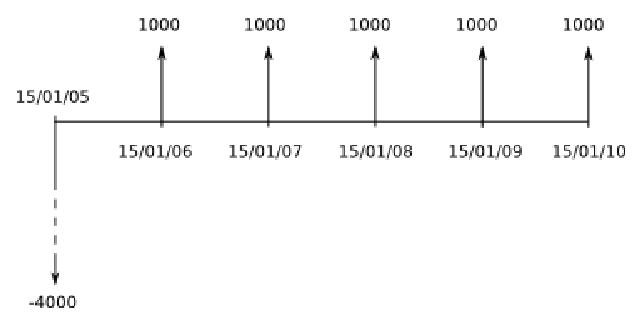
\includegraphics[width=7cm, angle=0]{./images/cashflow.eps}
\caption{Asset cashflow example}
\label{cashflow}
\end{center}
\end{figure}
\FloatBarrier

\paragraph{Recovery.} It is a ratio that indicates the portion of loss that will be recovered
in the case of default at a fixed time. This value takes into account guarantees, including 
the cost of taking legal action, and recovery rate based on historical data.
\newline

If a borrower defaults, the loss is the sum of all remaining cashflows at the default time 
(\emph{exposure}) as weighted by the recovery rate at the default time.

\begin{displaymath}
\mathrm{loss}_{t} = (1 - \mathrm{recovery}_t) \cdot \sum_{i \ge t} \mathrm{cashflow}_{i}
\end{displaymath}

\begin{figure}[!hbt]
\begin{center}
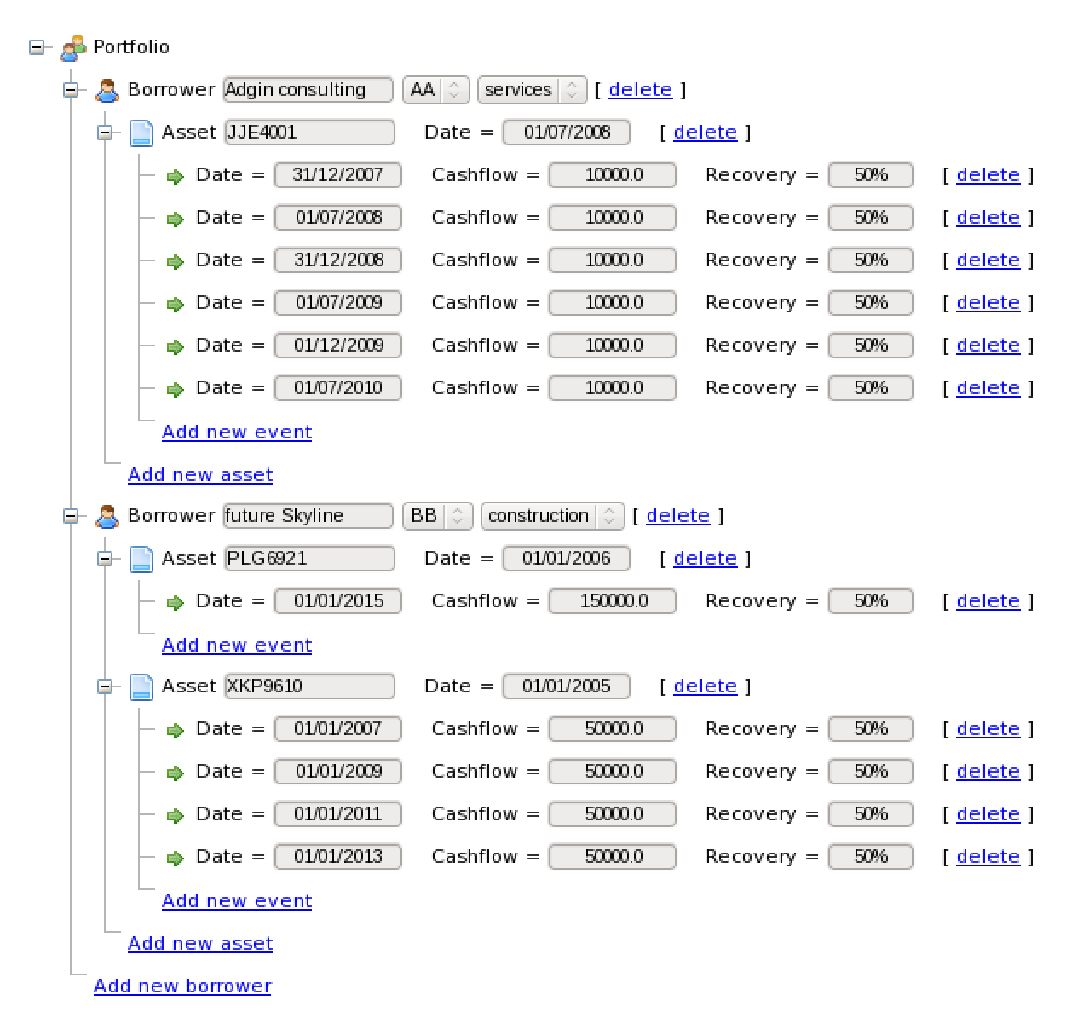
\includegraphics[height=10.5cm, angle=0]{./images/portfolio.eps}
\caption{Portfolio example}
\label{portfolio}
\end{center}
\end{figure}
\FloatBarrier

%===========================================================================
\clearpage
\section{Resolution}

This section explains how CCruncher computes the credit risk of a portfolio.
Figure \ref{fig:mcschema1} shows the schema followed to simulate the 
portfolio losses.

\begin{figure}[!hb]
\begin{center}
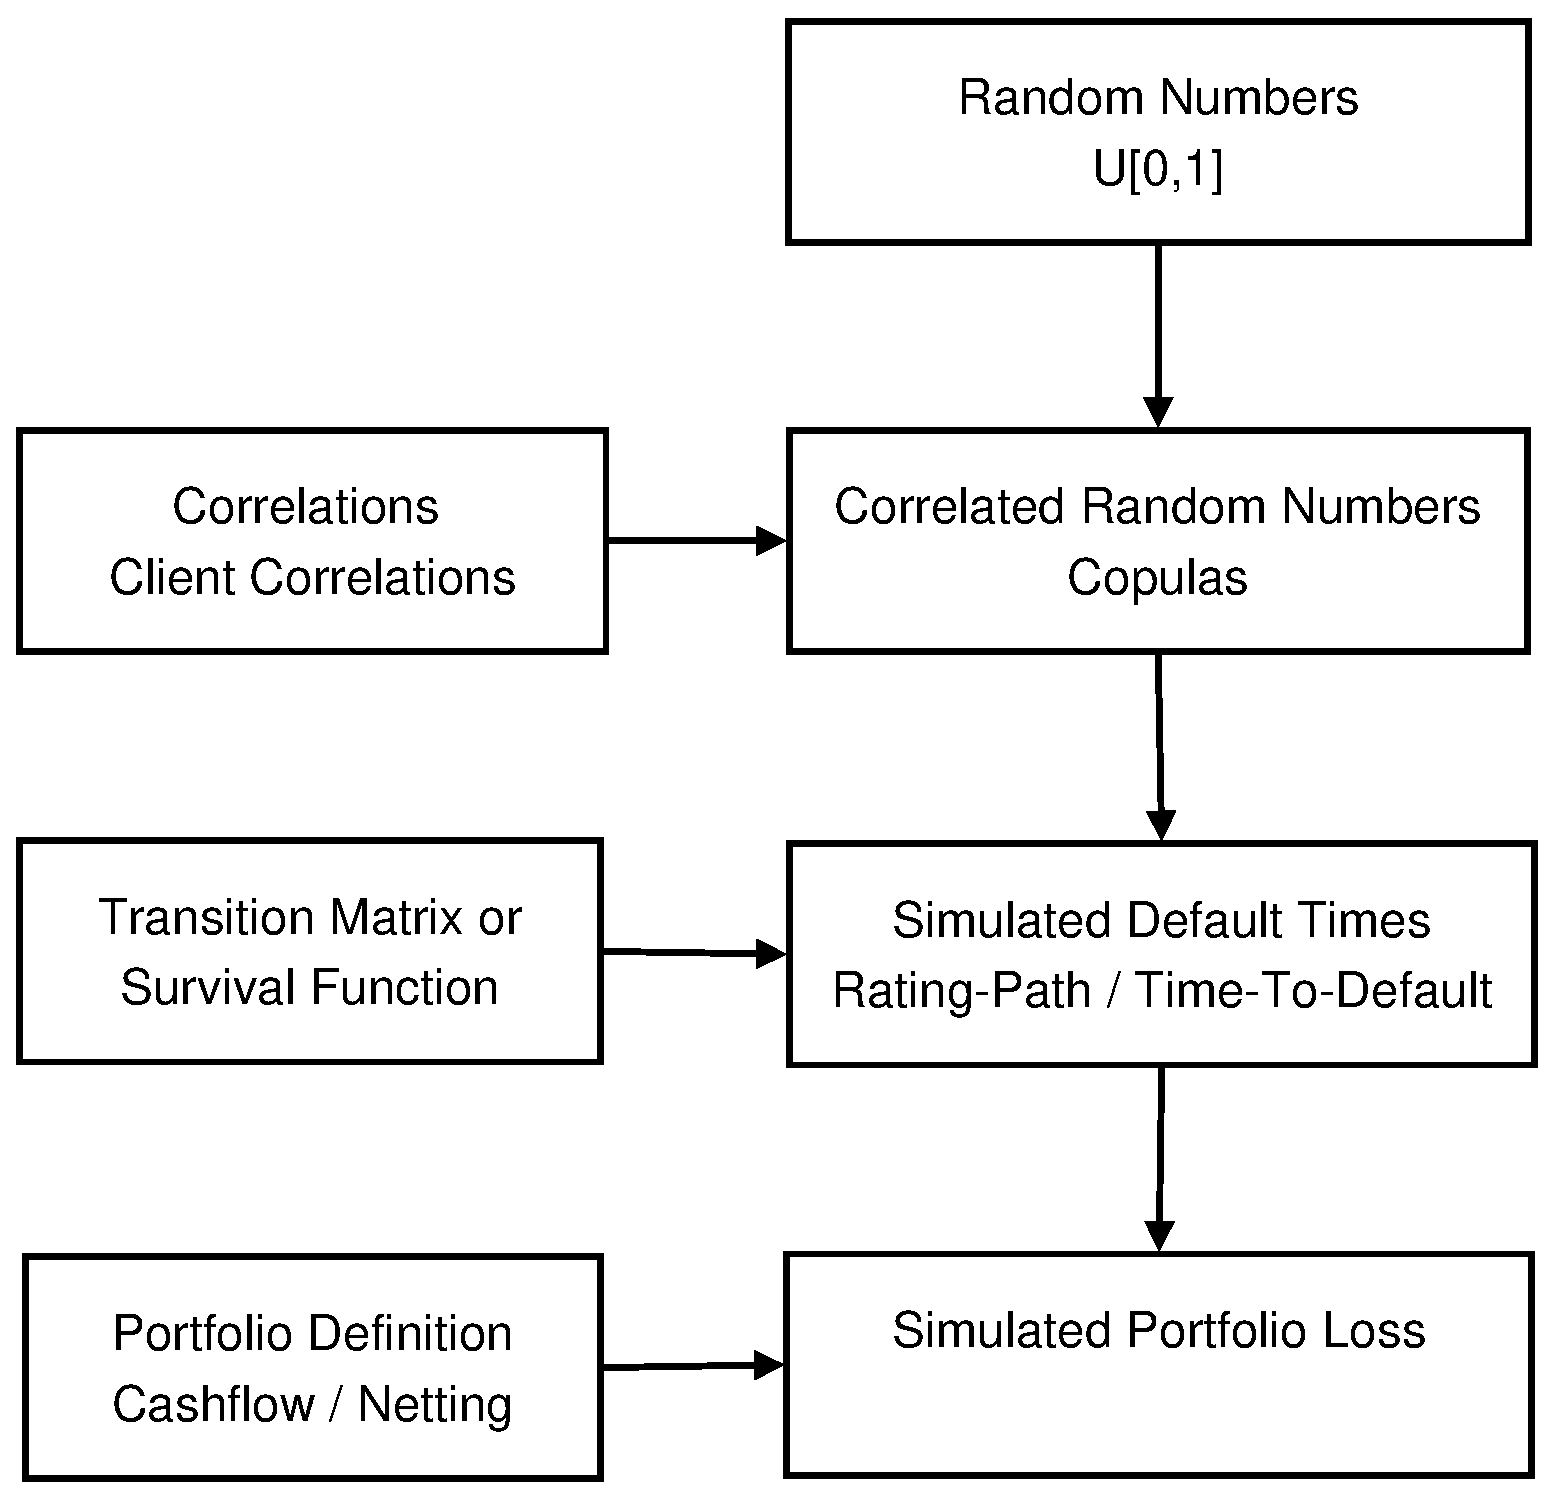
\includegraphics[width=10cm,angle=0]{./images/esquema1.eps}
\caption{Monte Carlo simulation schema}
\label{fig:mcschema1}
\end{center}
\end{figure}

%---------------------------------------------------------------------------
\subsection{Borrowers correlation matrix}
\label{tcorrel}
We need to translate from default correlations between sectors to default 
correlations between borrowers. Suppose we have $n$ borrowers and $m$ 
sectors. Each borrower belongs to a sector. $\rho_{i,j}$ are the estimated 
default time correlations between sectors:

\begin{center}
\begin{displaymath}
\begin{array}{cc}
\begin{array}{c|ccc}
                    & \mathrm{Sector}_1 & \dots  & \mathrm{Sector}_{m} \\
\hline
\mathrm{Sector}_1   & \rho_{1,1}        & \dots  & \rho_{1,m} \\
\vdots              & \vdots            & \ddots & \vdots     \\
\mathrm{Sector}_{m} & \rho_{1,m}        & \dots  & \rho_{m,m} \\
\end{array}
&
\qquad \rho_{i,j} = \mathrm{Corr}(\mathrm{Sector}_i, \mathrm{Sector}_j)
\end{array}
\end{displaymath}
\end{center}

Sort the borrowers so that those who belong to sector $1$ are at the beginning 
and those in sector $m$ are at the end. Then, create the borrowers correlation 
matrix, taking as the correlation between two borrowers the correlation between 
their sectors (see Figure \ref{borrowercorrel}).

\begin{figure}[!hb]
\begin{displaymath}
\begin{array}{c}
\Sigma=
\left(
\begin{array}{ccccccccccc}
1           & \dots    & \rho_{1,1}  &          & \rho_{1,k}  & \dots   & \rho_{1,k}  &         & \rho_{1,m}  & \dots      & \rho_{1,m}  \\
\vdots      & \ddots   & \vdots      &          & \vdots      &         & \vdots      &         & \vdots      &            & \vdots      \\
\rho_{1,1}  & \dots    & 1           &          & \rho_{1,k}  & \dots   & \rho_{1,k}  &         & \rho_{1,m}  & \dots      & \rho_{1,m}  \\

            &          &             & \ddots   &             &         &             &         &             &            &             \\

\rho_{1,k}  & \dots    & \rho_{1,k}  &          & 1           & \dots   & \rho_{k,k}  &         & \rho_{k,m}  & \dots      & \rho_{k,m}  \\
\vdots      & \ddots   & \vdots      &          & \vdots      & \ddots  & \vdots      &         & \vdots      &            & \vdots      \\
\rho_{1,k}  & \dots    & \rho_{1, }  &          & \rho_{k,k}  & \dots   & 1           &         & \rho_{k,m}  & \dots      & \rho_{k,m}  \\

            &          &             &          &             &         &             & \ddots  &             &            &             \\

\rho_{1,m}  & \dots    & \rho_{1,m}  &          & \rho_{k,m}  & \dots   & \rho_{k,m}  &         & 1           & \dots      & \rho_{m,m}  \\
\vdots      & \ddots   & \vdots      &          & \vdots      & \ddots  & \vdots      &         & \vdots      & \ddots     & \vdots      \\
\rho_{1,m}  & \dots    & \rho_{1,m}  &          & \rho_{k,m}  & \dots   & \rho_{k,m}  &         & \rho_{m,m}  & \dots      & 1           \\
\end{array}
\right)
\end{array}
\end{displaymath}
\caption{Borrowers correlation matrix}
\label{borrowercorrel}
\end{figure}

Observe that this is a correlation matrix (symmetric, $|\rho_{i,j}| \leq 1$, 
$\rho_{i,i} = 1$) that is composed of blocks. This matrix will be decomposed 
using the Cholesky algorithm, so it must be positive-definite.

%---------------------------------------------------------------------------
\subsection{Monte Carlo simulation}
\label{mcsim}
Monte Carlo methods are a class of computational algorithms for 
simulating the behaviour of various physical and mathematical systems. 
Each simulation consists of computing a random default time for each borrower 
and then calculating the loss of the portfolio. Default times must fulfil two 
conditions: the borrower's survival functions and the borrower's correlation 
matrix. The link between the marginal distributions (survival functions) and 
the dependence structure (correlations) is achieved with a copula.

\begin{comment}
TODO: The last two sentences do not clearly explain or make it obvious as to why 
a copula is needed for the default times to fulfill the two conditions. Maybe you 
could clarify those statements.
\end{comment}

%...........................................................................
\subsubsection{Correlated random numbers generation}
A copula \cite{copu:pitfalls} \cite{copu:wang} is a multivariate random variable 
in which each component is uniform, $U[0,1]$. Each simulation requires a set of 
random numbers between $[0, 1]$ and is correlated with the borrowers correlation 
matrix, $\Sigma$.

\begin{displaymath}
\begin{array}{ccc}
\begin{array}{|c|c|c|c|}
u_{11} & u_{12} & \dots  & u_{1n} \\
u_{21} & u_{22} & \dots  & u_{2n} \\
\vdots & \vdots & \vdots & \vdots \\
u_{k1} & u_{k2} & \dots  & u_{kn} \\
\end{array}
&
\qquad
&
\begin{array}{c}
n \textrm{ number of borrowers}    \\
k \textrm{ number of simulations}  \\
u_{.i} \sim U[0,1]                 \\
Corr(u_{.i}, u_{.j}) = \Sigma_{ij} \\
\end{array}
\end{array}
\end{displaymath}

Two copula generators, the Gaussian and the t-Student copulas, are implemented. 
These two copulas have good properties: they are commonly used in finance, exist 
algorithms to simulate them for any correlation matrix, and these algorithms work 
for large dimensions (see Appendices \ref{ap:gaussiancopu} and \ref{ap:tstudentcopu}).
\newline

Erik Kole et al. \cite{copu:selecting} have compared some copulas used in risk 
management. They observe that the t-Student copula can be considered to model the 
dependence between the different elements of a portfolio:
\begin{quotation}
"For a portfolio consisting of stocks, bonds and real estate, these tests provide
clear evidence in favor of the Student's t copula, and reject both the correlation-based
Gaussian copula and the extreme value-based Gumbel copula. In comparison with the
Student's t copula, we find that the Gaussian copula underestimates the probability of
joint extreme downward movements, while the Gumbel copula overestimates this risk.
Similarly we establish that the Gaussian copula is too optimistic on diversification
benefits, while the Gumbel copula is too pessimistic. Moreover, these differences are
significant."
\end{quotation}

%...........................................................................
\subsubsection{Default times simulation}
\label{sec:deftimessim}
Given a borrower $k$ and a random number ($u_k \in [0,1]$) (generated using a 
copula), we simulate the default time considering the inverse of the borrower 
survival function at $u_k$ \cite{ref:cred_risk}. 
Figure \ref{simttd} shows this graphically.

\begin{figure}[!hbt]
\begin{center}
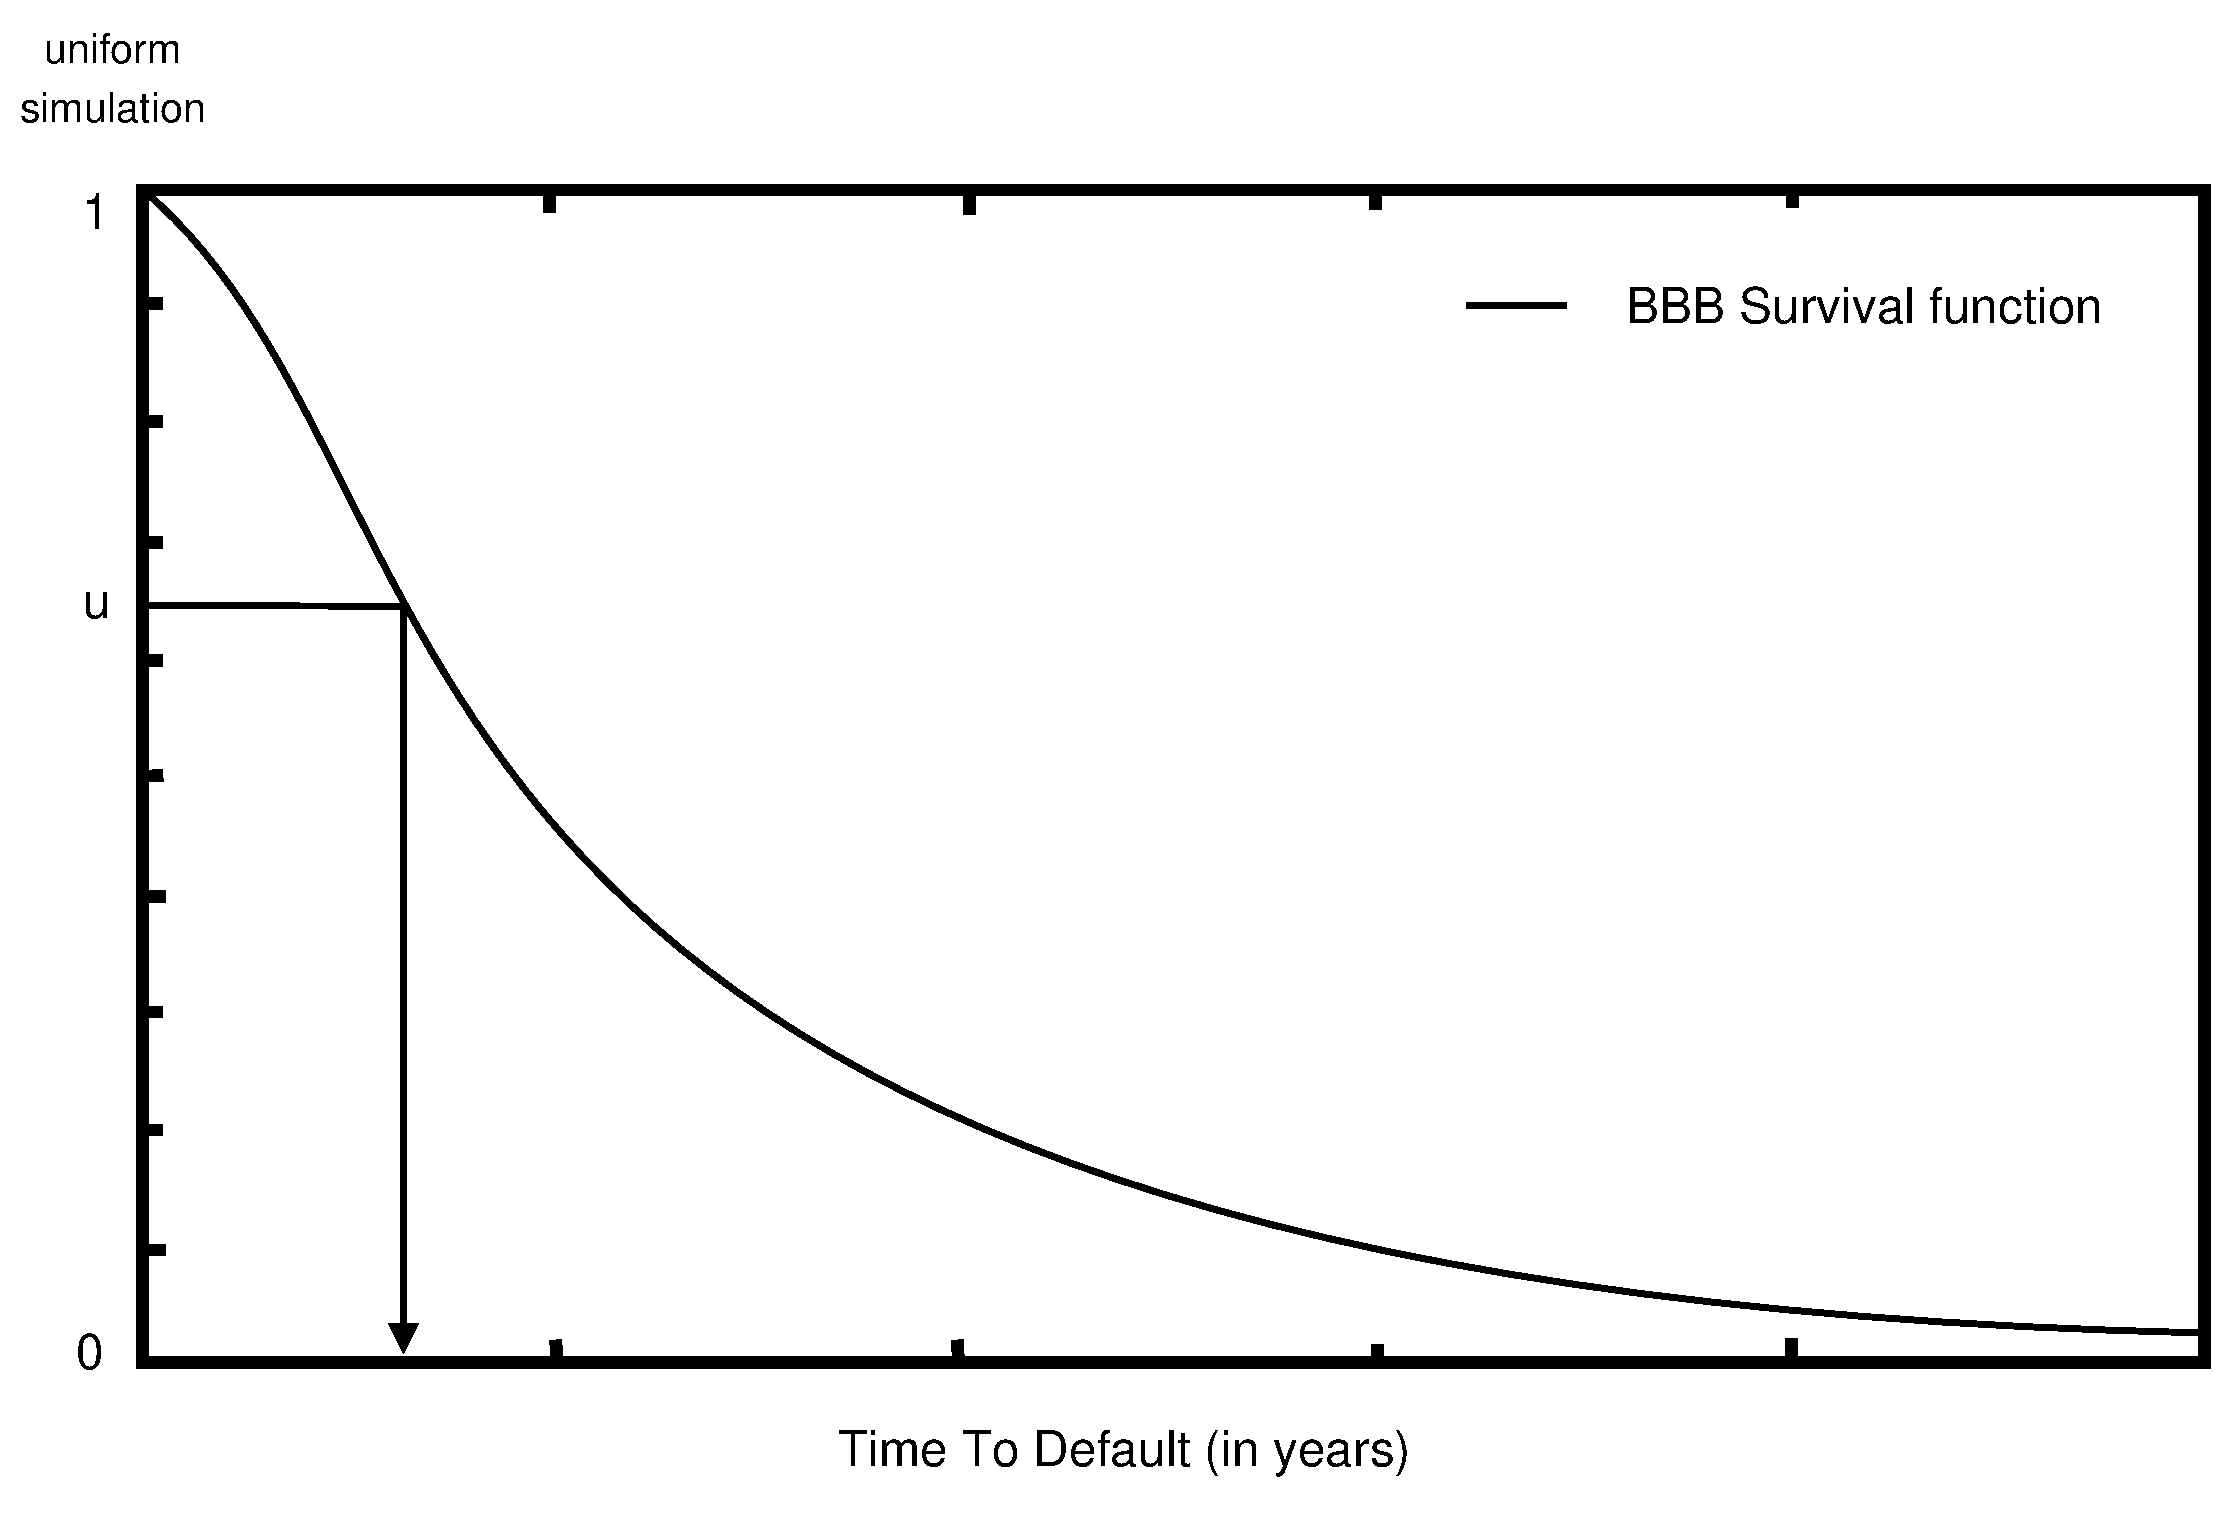
\includegraphics[width=10cm,angle=0]{./images/simttd.eps}
\caption{Default time generation with initial rating $BBB$}
\label{simttd}
\end{center}
\end{figure}
\FloatBarrier

%...........................................................................
\subsubsection{Portfolio loss evaluation}
\label{sec:portfolioloss}
At this point, all borrowers have a simulated default time. The loss
caused by any borrower is the sum of all remaining cashflows at the default time 
weighted by the recovery at the default time. To obtain the simulated 
value of the portfolio loss, add up all borrowers' losses:

\begin{displaymath}
\mathrm{PortfolioLoss} = \sum_{i=1}^N \mathrm{BorrowerLoss}_i
\end{displaymath}

where $N$ is the number of borrowers in the portfolio. For each borrower, we 
use the simulated default time, $t_i$, described in the previous section, to 
compute the borrower loss:

\begin{displaymath}
\mathrm{BorrowerLoss}_{i} = (1 - \mathrm{recovery}_{t_i}^i) \cdot \sum_{j \ge {t_i}} \mathrm{cashflow}_{j}^i
\end{displaymath}

%---------------------------------------------------------------------------
\subsection{Risk computation}
After $N$ simulations (eg. $20000$, $500000$ or more) we have a list
of numbers, ${x_1, ..., x_N}$, in which each number represents a simulated portfolio 
loss. The more values there are, the more accuracy there is in the results. All risk 
statistics (e.g., Expected Loss) have an error margin that will be estimated.
\newline

\begin{figure}[!hbt]
\begin{center}
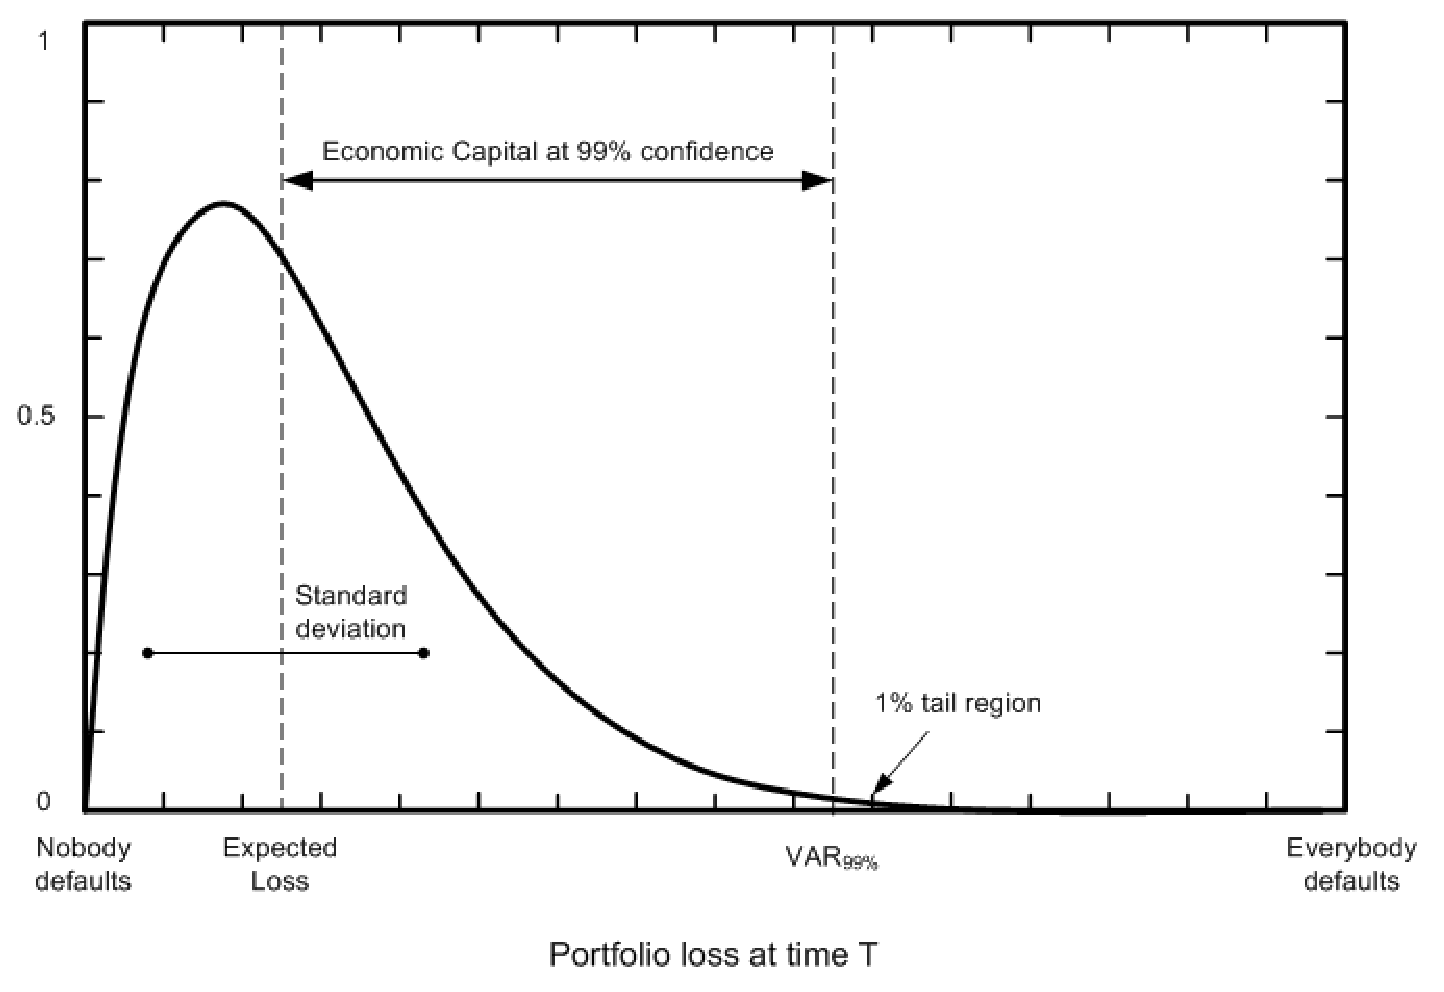
\includegraphics[height=7cm, angle=0]{./images/creditvar.eps}
\caption{Portfolio loss at time $T$}
\label{creditvar}
\end{center}
\end{figure}
\FloatBarrier

%...........................................................................
\subsubsection{Expected Loss}
The expected loss is the mean of the portfolio loss distribution.
The Central Limit Theorem \cite{stats:schaum} grants that:

\begin{displaymath}
\mu = \widehat{\mu} \pm \phi^{-1}\left(\frac{1-\alpha}{2}\right) \cdot \frac{\widehat{\sigma}}{\sqrt{N}}
\end{displaymath}
where $\alpha$ is the error confidence level, $\phi^{-1}$ is the $N(0,1)$ inverse 
cumulative distribution function, and $\widehat{\mu}$ and $\widehat{\sigma}$ are 
the mean and standard deviation estimators, respectively:

\begin{displaymath}
\widehat{\mu} = \frac{1}{N} \sum_{i=1}^{N} x_i
\end{displaymath}

\begin{displaymath}
\widehat{\sigma} =
\sqrt{\frac{1}{N-1} \sum_{i=1}^{N} \left( x_i - \widehat{\mu} \right)^2}
\end{displaymath}

%...........................................................................
\subsubsection{Portfolio Loss Standard Deviation}
Another usual risk statistic is the standard deviation of the portfolio loss.
The Central Limit Theorem \cite{stats:schaum} grants that:

\begin{displaymath}
\sigma = \widehat{\sigma} \pm \phi^{-1}\left(\frac{1-\alpha}{2}\right) \cdot \frac{\widehat{\sigma}}{\sqrt{2N}}
\end{displaymath}

where $\alpha$ is the error confidence level, $\phi^{-1}$ is the $N(0,1)$ inverse 
cumulative distribution function, and $\widehat{\sigma}$ is the standar deviation 
estimator that was defined previously.

%...........................................................................
\subsubsection{Value At Risk}
Value at Risk \cite{var:jorion} is the most commonly used risk value. We call it 
$\textrm{VAR}_{\beta}$ where $\beta$ is the VAR confidence level (e.g., VAR at $95\%$).
VAR is another way to say quantile. Thus,
$\textrm{VAR}_{\beta} = q_{\beta} = \textrm{inf}\{x | F(x) \geq \beta \}$ and

\begin{displaymath}
\textrm{VAR}_{\beta} = \widehat{q_{\beta}} \pm \phi^{-1}\left(\frac{1-\alpha}{2}\right) \cdot \textrm{stderr}(q_{\beta})
\end{displaymath}

where $\alpha$ is the error confidence level, $\beta$ is the VAR confidence 
level, $\phi^{-1}$ is the $N(0,1)$ inverse cumulative distribution function, 
$\widehat{q_{\beta}}$ is the quantile estimator, and $\textrm{stderr}(q_{\beta})$
is the estimation of the standard error.

\begin{displaymath}
\widehat{q_{\beta}} = x_{k:N}
\end{displaymath}
where
\begin{itemize}
\item $k$ fulfils $\frac{k}{N} \leq \beta < \frac{k+1}{N}$
\item $x_{k:N}$ is the $k$-th element of ascendant-sorted values.
\end{itemize}

Determine $\textrm{stderr}(q_{\beta})$ using the Maritz-Jarret method described
in \cite{quant:algor}:

\begin{displaymath}
\begin{array}{rcl}
M   & = & [N \beta + 0.5]  \\
a   & = & M - 1            \\
b   & = & N - M            \\
W_i & = & B(a,b,\frac{i+1}{N}) - B(a,b,\frac{i}{N}) \\
C_k & = & \sum_{i=1}^{N} W_i \cdot x_i^k \\
\end{array}
\end{displaymath}

where $[x]$ is the integer part of $x$ and $B(a,b,x)$ is the incomplete beta 
function:

\begin{displaymath}
B(a,b,x)=\frac{\Gamma(a+b)}{\Gamma(a)\Gamma(b)}\int_0^x t^{a-1} (1-t)^{b-1} dt
\end{displaymath}

Thus,
\begin{displaymath}
\textrm{stderr}(q_{\beta}) = \sqrt{C_2 - C_1^2}
\end{displaymath}

%...........................................................................
\subsubsection{Expected Shortfall}
VAR is not a distance because it does not fulfil the sub-additive property 
\cite{var:varbad}, $VAR(A+B) \nleq VAR(A)+VAR(B)$. Similar to VAR, Expected 
Shortfall is a consistent risk measure \cite{var:eshortfall}. It can be described
as the average of the $\beta\%$ worst losses:

\begin{displaymath}
ES_{\beta} = \widehat{ES_{\beta}} \pm \phi^{-1}\left(\frac{1-\alpha}{2}\right) \cdot \textrm{stderr}(ES_{\beta})
\end{displaymath}

where $\alpha$ is the error confidence level, $\beta$ is the ES confidence 
level, $\phi^{-1}$ is the $N(0,1)$ inverse cumulative distribution function, 
$\widehat{ES_{\beta}}$ is the ES estimator and $\textrm{stderr}(ES_{\beta})$
is the estimation of the standard error.
\newline

If we select the simulation portfolio loss values ($x_1, ..., x_N$) that are bigger 
than $VAR_{\beta}$,

\begin{displaymath}
y_1, y_2, y_3, \cdots, y_K \qquad \textrm{where} \quad y_i > VAR_{\beta}
\end{displaymath}

then,

\begin{displaymath}
\widehat{ES_{\beta}} = \frac{1}{K} \sum_{i=1}^{K} y_i
\end{displaymath}

\begin{displaymath}
\textrm{stderr}(ES_{\beta}) =
\frac{\sqrt{\frac{1}{K-1} \sum_{i=1}^{K} \left( y_i - \widehat{ES_{\beta}} \right)^2}}{\sqrt{K}}
\end{displaymath}

%...........................................................................
\subsubsection{Economic Capital}
Compute the Economic Capital at confidence level $\beta$ as:

\begin{displaymath}
\textrm{Economic Capital} = VAR_{\beta} - \textrm{Expected Loss}
\end{displaymath}

%...........................................................................

\begin{figure}[p]
\begin{center}
\includegraphics[width=12cm,angle=0]{./images/report.eps}
\caption{CCruncher results}
\label{report}
\end{center}
\end{figure}


%===========================================================================
\clearpage
\section{Other considerations}
CCruncher takes into consideration other concepts that have not been discussed 
up to this point with the purpose of simplifying the content.

%---------------------------------------------------------------------------
\subsection{Risk aggregation}
CCruncher simulates the whole portfolio loss at time $T$. It also allows (in 
the same execution) the simulation of subportfolios by defining one or more 
aggregators. Consequently, one can determine which borrowers (or products, 
branches, regions, assets, etc.) increase the risk of the portfolio. 
Each subportfolio has its own list of simulated values that can be processed to 
obtain the risk indicators for this subportfolio.

%---------------------------------------------------------------------------
\subsection{Yield curve}
CCruncher can consider that the value of money decreases with time, following a 
curve (e.g., a yield curve). CCruncher use this curve to compute the present value 
of the cash amounts. Allowed methods are simple interest, compound interest and
continuous interest.

%---------------------------------------------------------------------------
\subsection{Antithetic technique}
The random number generation using a copula is time intensive. The Gaussian and 
t-Student copulas are symmetric, which means that $(u_1, u_2, \cdots, u_n)$ is 
equiprobable to $(1-u_1, 1-u_2, \cdots, 1-u_n)$. In CCruncher's antithetic mode, 
each copula generation is used twice, $(u_1, u_2, \cdots, u_n)$ and 
$(1-u_1, 1-u_2, \cdots, 1-u_n)$, reducing by half the number of generated
copulas.

%---------------------------------------------------------------------------
\subsection{Parallel computing}
Monte Carlo problems are embarrassingly parallel problems.
In the jargon of parallel computing, an embarrassingly parallel workload 
(or embarrassingly parallel problem) is one for which no particular effort 
is needed to segment the problem into a very large number of parallel tasks, 
and there is no essential dependency (or communication) among those parallel 
tasks.
\newline

In CCruncher, the master sends a distinct seed to each slave to initialize its RNG 
and waits for results (the simulated values of the portfolio loss) from slaves that 
store them in a file. When one of the two stop criteria is achieved (the maximum 
execution time or the maximum number of simulations are exceeded), the master sends 
a stop signal to the slaves and leaves.


%===========================================================================
\pagebreak
\section{Numerical example}

We compute the credit risk at $T=30$ years for the following portfolio.

\begin{table}[!h]
\begin{center}
\begin{tabular}[]{c|l|c|c|c|l}
Id  & Borrower name        & Rating & Sector         & Recovery & Assets     \\
\hline
B1  & Future Skyline       & AA     & Construction   & 80\%     & A1         \\
B2  & Ramses builds        & BBB    & Construction   & 75\%     & A2, A3     \\
B3  & Gramdateresi         & AA     & Consumer goods & 60\%     & A4         \\
B4  & Tantor Pinori        & BB     & Consumer goods & 90\%     & A5, A6, A7 \\
B5  & White \& Rebolan     & B      & Services       & 30\%     & A8         \\
B6  & Adign Consulting     & BBB    & Services       & 60\%     & A9         \\
B7  & Advanced Engineering & AAA    & Services       & 50\%     & A10        \\
B8  & Sigmacle Research    & CCC    & Services       & 60\%     & A11        \\
B9  & Loglament Asia       & AA     & Services       & 50\%     & A12        \\
\end{tabular}
\caption{Portfolio composition}
\label{example.portfolio}
\end{center}
\end{table}

The following table lists the asset events in months from the current date.

{\small
\begin{table}[!h]
\begin{center}
\begin{tabular}[]{c|c|c|c|c|c|c|c|c|c|c|c|c}
Month & A1  & A2  & A3  & A4  & A5  & A6  & A7  & A8  & A9  & A10 & A11 & A12  \\
\hline
6     & 10\$&     &     &     &100\$&     &     &     &     &     &     & 70\$ \\
12    &     & 50\$&     &     &     & 20\$& 80\$&     & 20\$&     &     &      \\
36    &     &     &     &     &     &     &     &     &     &     & 30\$&      \\
60    &     & 30\$&     &     & 10\$&     & 20\$& 80\$&     &     &     &      \\
90    &     &     &     &     &     & 30\$&     &     &     &     &     &      \\
120   & 15\$&     & 40\$&     & 30\$&     &     &     &     &     &     &      \\
180   &     &     &     &     & 40\$& 70\$&     &     &     &     &     &      \\
216   &     & 10\$&     &     & 50\$&     &     &     &     &     &     & 80\$ \\
240   &     &     &     &100\$&     &     &     &     &     &     &     &      \\
312   &100\$&     & 40\$&     & 70\$&     &     &     & 70\$&     &     &      \\
360   &     &     &     &     &     & 15\$&     &     &     &     & 40\$&      \\
384   & 90\$&     &     &     & 90\$&     &     &     &     &100\$& 90\$&      \\       
\end{tabular}
\caption{Asset events}
\label{example.assets}
\end{center}
\end{table}
}

This example assumes that there are no survival functions, but we have the 
one-year transition matrix $T_1$ (extracted from \cite{CreditMetrics:Tech_Doc}).

\begin{table}[!h]
\begin{center}
\begin{tabular}[]{l|rrrrrrrr}
        &      AAA &       AA &        A &      BBB &       BB &        B &      CCC &  Default \\
\hline
AAA     &  $90.81$ &   $8.33$ &   $0.68$ &   $0.06$ &   $0.12$ &   $0.00$ &   $0.00$ &   $0.00$ \\
 AA     &   $0.70$ &  $90.65$ &   $7.79$ &   $0.64$ &   $0.06$ &   $0.14$ &   $0.02$ &   $0.00$ \\
  A     &   $0.09$ &   $2.27$ &  $91.05$ &   $5.52$ &   $0.74$ &   $0.26$ &   $0.01$ &   $0.06$ \\
BBB     &   $0.02$ &   $0.33$ &   $5.95$ &  $86.93$ &   $5.30$ &   $1.17$ &   $0.12$ &   $0.18$ \\
 BB     &   $0.03$ &   $0.14$ &   $0.67$ &   $7.73$ &  $80.53$ &   $8.84$ &   $1.00$ &   $1.06$ \\
  B     &   $0.00$ &   $0.11$ &   $0.24$ &   $0.43$ &   $6.48$ &  $83.46$ &   $4.07$ &   $5.21$ \\
CCC     &   $0.22$ &   $0.00$ &   $0.22$ &   $1.30$ &   $2.38$ &  $11.24$ &  $64.86$ &  $19.78$ \\
Default &   $0.00$ &   $0.00$ &   $0.00$ &   $0.00$ &   $0.00$ &   $0.00$ &   $0.00$ & $100.00$ \\
\end{tabular}
\caption{One-year transition matrix}
\label{example.tmatrix}
\end{center}
\end{table}
\FloatBarrier

The sectorial default time correlations are:

\begin{table}[!h]
\begin{center}
\begin{tabular}[]{l|ccc}
               & Construction & Consumer goods & Services \\
\hline
Construction   &    $0.50$    &     $0.20$     &   $0.30$ \\
Consumer goods &    $0.20$    &     $0.60$     &   $0.34$ \\
Services       &    $0.30$    &     $0.34$     &   $0.40$ \\
\end{tabular}
\caption{Sector correlation matrix}
\label{example.scorrels}
\end{center}
\end{table}
\FloatBarrier

%---------------------------------------------------------------------------
\subsection{Obtaining the survival functions}

Appendix \ref{ap:tmatrix} is used to compute the survival functions 
with a time resolution of one month. We scale\footnote{CAUTION: 
calculations should be performed using absolute values, not percentages.}
the transition matrix to one month by using $T_{\frac{1}{12}} = T_{1}^{\frac{1}{12}}$.  
The one-month transition matrix, $T_{\frac{1}{12}}$, is given by:
{\small
\begin{displaymath}
%T_{\frac{1}{12}} = 
\left( 
\begin{array}{cccccccc}
    99.1972  &   0.7588  &   0.0320  &   0.0020  &   0.0112  &  -0.0011  &  -0.0001  &   0.0000  \\
     0.0635  &  99.1745  &   0.7083  &   0.0392  &   0.0015  &   0.0120  &   0.0018  &  -0.0007  \\
     0.0074  &   0.2057  &  99.1980  &   0.5102  &   0.0557  &   0.0189  &  -0.0001  &   0.0042  \\
     0.0015  &   0.0239  &   0.5507  &  98.8021  &   0.5164  &   0.0871  &   0.0077  &   0.0107  \\
     0.0027  &   0.0113  &   0.0396  &   0.7581  &  98.1558  &   0.8774  &   0.0889  &   0.0664  \\
    -0.0007  &   0.0098  &   0.0196  &   0.0111  &   0.6447  &  98.4443  &   0.4463  &   0.4249  \\
     0.0233  &  -0.0023  &   0.0170  &   0.1287  &   0.2166  &   1.2298  &  96.4213  &   1.9657  \\
     0.0000  &   0.0000  &   0.0000  &   0.0000  &   0.0000  &   0.0000  &   0.0000  & 100.0000  \\
\end{array}
\right)
\end{displaymath}
}

Note the negative values in the computed one-month transition matrix. 
These values result from the fact that the original matrix ($T_1$) is not a regular Markov matrix. 
In these cases, CCruncher regularizes the matrix by applying the algorithm described in Appendix 
\ref{ap:regularization}. To simplify this example, the negative values are replaced by $0$.
\newline

Compute the survival values at month one by using the one-month transition matrix 
(the $d$ subindex means the default column):
\begin{displaymath}
S(.,1 \textrm{ month}) = \vec{1} - (T_{1/12})_{.d} = 
\left( 
\begin{array}{c}
 100 \\
 100 \\
 100 \\
 100 \\
 100 \\
 100 \\
 100 \\
\end{array}
\right)
 - 
\left( 
\begin{array}{c}
 0.0000 \\
 0.0000 \\
 0.0042 \\
 0.0107 \\
 0.0664 \\
 0.4249 \\
 1.9657 \\
\end{array}
\right)
=
\left( 
\begin{array}{c}
 100.000 \\
 100.000 \\
  99.996 \\
  99.989 \\
  99.934 \\
  99.975 \\
  98.034 \\
\end{array}
\right)
\end{displaymath}

Then, compute the survival values at month two:
\begin{displaymath}
S(.,2 \textrm{ months}) = \vec{1} - (T_{1/12}^2)_{.d} = 
\left( 
\begin{array}{c}
 100 \\
 100 \\
 100 \\
 100 \\
 100 \\
 100 \\
 100 \\
\end{array}
\right)
 - 
\left( 
\begin{array}{c}
 0.0000 \\
 0.0000 \\
 0.0084 \\
 0.0221 \\
 0.1372 \\
 0.8524 \\
 3.8664 \\
\end{array}
\right)
=
\left( 
\begin{array}{c}
 100.000 \\
 100.000 \\
  99.992 \\
  99.978 \\
  99.863 \\
  99.148 \\
  96.134 \\
\end{array}
\right)
\end{displaymath}

Next, compute the survivals values at month three:

\begin{displaymath}
S(.,3 \textrm{ months}) = \vec{1} - (T_{1/12}^3)_{.d} = 
\left( 
\begin{array}{c}
 100 \\
 100 \\
 100 \\
 100 \\
 100 \\
 100 \\
 100 \\
\end{array}
\right)
 - 
\left( 
\begin{array}{c}
 0.0000 \\
 0.0000 \\
 0.0129 \\
 0.0342 \\
 0.2122 \\
 1.2821 \\
 5.7045 \\
\end{array}
\right)
=
\left( 
\begin{array}{c}
 100.000 \\
 100.000 \\
  99.987 \\
  99.966 \\
  99.788 \\
  98.718 \\
  94.296 \\
\end{array}
\right)
\end{displaymath}

Repeat the same procedure for $360$ months to obtain the survival
functions shown in Table \ref{example.survivals}.

\clearpage 

\begin{table}[!hb]
\begin{center}
{\small
\begin{tabular}[]{c|rrrrrrrr}
Month &  AAA   &  AA    &   A    &  BBB   &  BB    &   B    &  CCC   \\
\hline
1   & 100.000 & 100.000 &  99.996 &  99.989 &  99.934 &  99.575 &  98.034 \\
2   & 100.000 & 100.000 &  99.992 &  99.978 &  99.863 &  99.148 &  96.134 \\
3   & 100.000 & 100.000 &  99.987 &  99.966 &  99.788 &  98.718 &  94.296 \\
4   & 100.000 & 100.000 &  99.983 &  99.953 &  99.709 &  98.286 &  92.518 \\
5   & 100.000 & 100.000 &  99.978 &  99.939 &  99.626 &  97.853 &  90.798 \\
6   & 100.000 & 100.000 &  99.973 &  99.925 &  99.539 &  97.418 &  89.134 \\
7   & 100.000 & 100.000 &  99.968 &  99.909 &  99.448 &  96.981 &  87.525 \\
8   & 100.000 & 100.000 &  99.963 &  99.893 &  99.353 &  96.544 &  85.967 \\
9   & 100.000 & 100.000 &  99.957 &  99.876 &  99.255 &  96.106 &  84.460 \\
10  & 100.000 & 100.000 &  99.952 &  99.858 &  99.153 &  95.668 &  83.000 \\
11  & 100.000 & 100.000 &  99.946 &  99.840 &  99.048 &  95.229 &  81.588 \\
12  & 100.000 & 100.000 &  99.940 &  99.820 &  98.940 &  94.790 &  80.220 \\
13  & 100.000 &  99.999 &  99.934 &  99.800 &  98.828 &  94.351 &  78.896 \\
14  & 100.000 &  99.998 &  99.928 &  99.778 &  98.714 &  93.912 &  77.613 \\
15  & 100.000 &  99.997 &  99.921 &  99.756 &  98.596 &  93.474 &  76.370 \\
\ldots & \ldots & \ldots & \ldots & \ldots & \ldots & \ldots & \ldots \\
169 &  99.213 &  97.964 &  95.345 &  88.888 &  72.479 &  50.213 &  28.155 \\
170 &  99.200 &  97.936 &  95.292 &  88.793 &  72.333 &  50.062 &  28.073 \\
171 &  99.187 &  97.908 &  95.240 &  88.698 &  72.188 &  49.912 &  \underline{27.992} \\
172 &  99.173 &  97.880 &  95.187 &  88.604 &  72.043 &  49.764 &  27.911 \\
173 &  99.159 &  97.851 &  95.134 &  88.509 &  71.899 &  49.616 &  27.832 \\
\ldots & \ldots & \ldots & \ldots & \ldots & \ldots & \ldots & \ldots \\
308 &  95.906 &  92.251 &  86.516 &  76.085 &  56.684 &  35.993 &  20.548 \\
309 &  95.871 &  92.198 &  86.445 &  75.999 &  56.596 &  35.924 &  20.511 \\
310 &  95.837 &  92.145 &  86.375 &  75.913 &  \underline{56.509} &  35.855 &  20.474 \\
311 &  95.801 &  92.093 &  86.304 &  75.828 &  56.423 &  35.787 &  20.437 \\
312 &  95.766 &  92.040 &  86.234 &  75.742 &  56.336 &  35.719 &  20.400 \\
\ldots & \ldots & \ldots & \ldots & \ldots & \ldots & \ldots & \ldots \\
358 &  93.986 &  89.478 &  82.955 &  71.932 &  52.638 &  32.889 &  18.868 \\
359 &  93.944 &  89.419 &  82.883 &  71.851 &  52.563 &  32.833 &  18.838 \\
360 &  93.902 &  89.361 &  82.812 &  71.771 &  52.488 &  32.778 &  18.808 \\
\end{tabular}
}
\caption{Survival functions table}
\label{example.survivals}
\end{center}
\end{table}

\clearpage 

%---------------------------------------------------------------------------
\subsection{Creating the borrowers correlation matrix}

Use Section \ref{tcorrel} to create the borrowers correlation matrix. In 
this example, the debtors are sorted by sector, and therefore, no reorder is 
required.
\begin{displaymath}
\Sigma = 
\left( 
\begin{array}{cc|cc|ccccc}
 1.00 & 0.50 & 0.20 & 0.20 & 0.30 & 0.30 & 0.30 & 0.30 & 0.30 \\
 0.50 & 1.00 & 0.20 & 0.20 & 0.30 & 0.30 & 0.30 & 0.30 & 0.30 \\
\hline
 0.20 & 0.20 & 1.00 & 0.60 & 0.34 & 0.34 & 0.34 & 0.34 & 0.34 \\
 0.20 & 0.20 & 0.60 & 1.00 & 0.34 & 0.34 & 0.34 & 0.34 & 0.34 \\
\hline
 0.30 & 0.30 & 0.34 & 0.34 & 1.00 & 0.40 & 0.40 & 0.40 & 0.40 \\
 0.30 & 0.30 & 0.34 & 0.34 & 0.40 & 1.00 & 0.40 & 0.40 & 0.40 \\
 0.30 & 0.30 & 0.34 & 0.34 & 0.40 & 0.40 & 1.00 & 0.40 & 0.40 \\
 0.30 & 0.30 & 0.34 & 0.34 & 0.40 & 0.40 & 0.40 & 1.00 & 0.40 \\
 0.30 & 0.30 & 0.34 & 0.34 & 0.40 & 0.40 & 0.40 & 0.40 & 1.00 \\
\end{array}
\right)
\end{displaymath}

%---------------------------------------------------------------------------
\subsection{Copula initialization}

In this example, we simulate the default times using a Gaussian copula. 
We compute the covariance matrix, $\Sigma'$, following Steps $1$ and $2$ 
in Appendix \ref{ap:gaussiancopu}.
\newline

Create the covariance matrix $\Sigma'$ by mapping each $\Sigma$ component, 
$\rho_{ij}$, to $2 sin(\frac{\pi}{6} \rho_{ij})$:
{\small
\begin{displaymath}
\Sigma' = 
\left( 
\begin{array}{ccccccccc}
   1.0000 & 0.5176 & 0.2091 & 0.2091 & 0.3129 & 0.3129 & 0.3129 & 0.3129 & 0.3129 \\
   0.5176 & 1.0000 & 0.2091 & 0.2091 & 0.3129 & 0.3129 & 0.3129 & 0.3129 & 0.3129 \\
   0.2091 & 0.2091 & 1.0000 & 0.6180 & 0.3542 & 0.3542 & 0.3542 & 0.3542 & 0.3542 \\
   0.2091 & 0.2091 & 0.6180 & 1.0000 & 0.3542 & 0.3542 & 0.3542 & 0.3542 & 0.3542 \\
   0.3129 & 0.3129 & 0.3542 & 0.3542 & 1.0000 & 0.4158 & 0.4158 & 0.4158 & 0.4158 \\
   0.3129 & 0.3129 & 0.3542 & 0.3542 & 0.4158 & 1.0000 & 0.4158 & 0.4158 & 0.4158 \\
   0.3129 & 0.3129 & 0.3542 & 0.3542 & 0.4158 & 0.4158 & 1.0000 & 0.4158 & 0.4158 \\
   0.3129 & 0.3129 & 0.3542 & 0.3542 & 0.4158 & 0.4158 & 0.4158 & 1.0000 & 0.4158 \\
   0.3129 & 0.3129 & 0.3542 & 0.3542 & 0.4158 & 0.4158 & 0.4158 & 0.4158 & 1.0000 \\
\end{array}
\right)
\end{displaymath}
}

Next, apply Cholesky to $\Sigma'$. Then $\Sigma' = B \cdot B^{\top}$, where:
{\small
\begin{displaymath}
B = 
\left(
\begin{array}{ccccccccc}
   1.0000 & 0.0000 & 0.0000 & 0.0000 & 0.0000 & 0.0000 & 0.0000 & 0.0000 & 0.0000 \\
   0.5176 & 0.8556 & 0.0000 & 0.0000 & 0.0000 & 0.0000 & 0.0000 & 0.0000 & 0.0000 \\
   0.2091 & 0.1179 & 0.9708 & 0.0000 & 0.0000 & 0.0000 & 0.0000 & 0.0000 & 0.0000 \\
   0.2091 & 0.1179 & 0.5773 & 0.7805 & 0.0000 & 0.0000 & 0.0000 & 0.0000 & 0.0000 \\
   0.3129 & 0.1764 & 0.2760 & 0.1392 & 0.8806 & 0.0000 & 0.0000 & 0.0000 & 0.0000 \\
   0.3129 & 0.1764 & 0.2760 & 0.1392 & 0.2172 & 0.8534 & 0.0000 & 0.0000 & 0.0000 \\
   0.3129 & 0.1764 & 0.2760 & 0.1392 & 0.2172 & 0.1688 & 0.8365 & 0.0000 & 0.0000 \\
   0.3129 & 0.1764 & 0.2760 & 0.1392 & 0.2172 & 0.1688 & 0.1382 & 0.8250 & 0.0000 \\
   0.3129 & 0.1764 & 0.2760 & 0.1392 & 0.2172 & 0.1688 & 0.1382 & 0.1170 & 0.8167 \\
\end{array}
\right)
\end{displaymath}
}

%---------------------------------------------------------------------------
\subsection{Monte Carlo simulation}

Each Monte Carlo trial consists of three parts: the copula simulation, the default 
times simulation and the portfolio loss evaluation.

\paragraph{Copula simulation.} To simulate the Gaussian copula, we follow  
Steps $3$ to $5$ in Appendix \ref{ap:gaussiancopu}. To simulate the multivariate
$\vec{Z} \sim N(0,\Sigma')$, simulate nine independent $N(0,1)$ variables and 
multiply by $B$.
{\small
\begin{displaymath}
\vec{Z} = B \cdot
\left(
\begin{array}{c}
  +0.0689 \\
  -0.3096 \\
  -0.2790 \\
  +0.4435 \\
  -1.2855 \\
  -0.8553 \\
  -0.6456 \\
  -0.0275 \\
  -0.6733 \\
\end{array}
\right) 
=
\left(
\begin{array}{c}
  +0.0689 \\
  -0.2292 \\
  -0.2929 \\
  +0.1630 \\
  -1.1803 \\
  -1.0575 \\
  -1.0120 \\
  -0.5839 \\
  -1.1143 \\
\end{array}
\right) 
\end{displaymath}
}

Finally, obtain the copula $\vec{U}$ in the following way:
{\small
\begin{displaymath}
\vec{U} 
=
\left(
\begin{array}{c}
\Phi(+0.0689) \\
\Phi(-0.2292) \\
\Phi(-0.2929) \\
\Phi(+0.1630) \\
\Phi(-1.1803) \\
\Phi(-1.0575) \\
\Phi(-1.0120) \\
\Phi(-0.5839) \\
\Phi(-1.1143) \\
\end{array}
\right) 
=
\left(
\begin{array}{c}
   0.5275 \\
   0.4093 \\
   0.3848 \\
   0.5647 \\
   0.1189 \\
   0.1452 \\
   0.1558 \\
   0.2797 \\
   0.1326 \\
\end{array}
\right) 
\end{displaymath}
}
where $\Phi(x)$ is the $N(0,1)$ cumulative distribution function.

\paragraph{Default times simulation.} To simulate the default time, use the 
inverse of the survival functions, as explained in Section \ref{sec:deftimessim}.
The first borrower has an initial rating AA and a copula value of $52.75$. 
In Table \ref{example.survivals} search for the month in which AA is close to 
$52.75$, and consider this month, $961$, as the month in which the first borrower 
defaults. 
{\small
\begin{table}[!hbt]
\begin{center}
\begin{tabular}[]{|c|c|c|c|}
Borrower & Rating & $\vec{U}_i$ & Default month \\
\hline
B1       & AA     &  0.5275     &  961      \\
B2       & BBB    &  0.4093     &  898      \\
B3       & AA     &  0.3848     &  $>$ 1000 \\
B4       & BB     &  0.5647     &  310      \\
B5       & B      &  0.1189     &  $>$ 1000 \\
B6       & BBB    &  0.1452     &  $>$ 1000 \\
B7       & AAA    &  0.1558     &  $>$ 1000 \\
B8       & CCC    &  0.2797     &  171      \\
B9       & AA     &  0.1326     &  $>$ 1000 \\
\end{tabular}
\caption{Simulated default times}
\end{center}
\end{table}
}
\FloatBarrier

\paragraph{Portfolio loss evaluation.} To evaluate the portfolio loss, 
we use the simulated default times and the portfolio composition (Tables 
\ref{example.portfolio} and \ref{example.assets}), as explained in Section 
\ref{sec:portfolioloss}.
{\small
\begin{table}[!hbt]
\begin{center}
\begin{tabular}[]{|c|c|c|c|c|c|}
Borrower & Default month & Asset & Exposure    & Recovery & Loss  \\
\hline
B1       & 961           &  A1   &             &  80\%    &       \\
B2       & 898           &  A2   &             &  75\%    &       \\
B2       & 898           &  A3   &             &  75\%    &       \\
B3       & $>$ 1000      &  A4   &             &  60\%    &       \\
B4       & 310           &  A5   & 70\$ + 90\$ &  90\%    &  16\$ \\
B4       & 310           &  A6   & 15\$        &  90\%    & 1.5\$ \\
B4       & 310           &  A7   &             &  90\%    &       \\
B5       & $>$ 1000      &  A8   &             &  30\%    &       \\
B6       & $>$ 1000      &  A9   &             &  60\%    &       \\
B7       & $>$ 1000      &  A10  &             &  50\%    &       \\
B8       & 171           &  A11  & 40\$ + 90\$ &  60\%    &  52\$ \\
B9       & $>$ 1000      &  A12  &             &  50\%    &       \\
\end{tabular}
\caption{Portfolio loss evaluation}
\end{center}
\end{table}
}

The simulated portfolio loss is the sum of all asset losses, or \$ $69.5$ 
in this Monte Carlo trial. 

\FloatBarrier


%===========================================================================
\begin{comment}
\section{Case studies}

\subsection{Identical uncorrelated borrowers}
%TODO: fill this section. use samples/README

\subsection{Identical correlated borrowers}
%TODO: fill this section. use samples/README

\subsection{Non-identical uncorrelated borrowers}
%TODO: fill this section. use samples/README

\subsection{Non-identical correlated borrowers}
%TODO: fill this section. use samples/README
\end{comment}

%===========================================================================
\newpage
\appendix
\section{Appendices}

%---------------------------------------------------------------------------
\subsection{From transition matrix to survival functions}
\label{ap:tmatrix}
The $T$-years transition matrix gives the probability of changing from rating $r_i$ 
to rating $r_j$ in a period of $T$ years:

\begin{displaymath}
M_T = \left(
\begin{array}{ccc}
m_{1,1} & \dots  & m_{1,n} \\
\vdots & \ddots & \vdots   \\
m_{n,1} & \dots  & m_{n,n} \\
\end{array}
\right)
\qquad
m_{i,j} = P(r_i \to r_j;T)
\end{displaymath}

where $n$ is the number of ratings and $m_{i,j}$ is the probability that a
borrower with rating $r_i$ changes to rating $r_j$ in $T$ years.
Figure \ref{tmatrix1} shows a transition matrix in which the probability that 
a borrower with rating $AA$ changes to rating $B$ in one year is $0.14\%$.
\newline

\begin{figure}[!hb]
\begin{center}
\begin{tabular}[]{l|rrrrrrrr}
        &      AAA &       AA &        A &      BBB &       BB &        B &      CCC &  Default \\
\hline
AAA     &  $90.81$ &   $8.33$ &   $0.68$ &   $0.06$ &   $0.12$ &   $0.00$ &   $0.00$ &   $0.00$ \\
 AA     &   $0.70$ &  $90.65$ &   $7.79$ &   $0.64$ &   $0.06$ &   $\underline{0.14}$ &   $0.02$ &   $0.00$ \\
  A     &   $0.09$ &   $2.27$ &  $91.05$ &   $5.52$ &   $0.74$ &   $0.26$ &   $0.01$ &   $0.06$ \\
BBB     &   $0.02$ &   $0.33$ &   $5.95$ &  $86.93$ &   $5.30$ &   $1.17$ &   $0.12$ &   $0.18$ \\
 BB     &   $0.03$ &   $0.14$ &   $0.67$ &   $7.73$ &  $80.53$ &   $8.84$ &   $1.00$ &   $1.06$ \\
  B     &   $0.00$ &   $0.11$ &   $0.24$ &   $0.43$ &   $6.48$ &  $83.46$ &   $4.07$ &   $5.21$ \\
CCC     &   $0.22$ &   $0.00$ &   $0.22$ &   $1.30$ &   $2.38$ &  $11.24$ &  $64.86$ &  $19.78$ \\
Default &   $0.00$ &   $0.00$ &   $0.00$ &   $0.00$ &   $0.00$ &   $0.00$ &   $0.00$ & $100.00$ \\
\end{tabular}
\caption{One-year transition matrix}
\label{tmatrix1}
\end{center}
\end{figure}

The transition matrix can be scaled in time by using the following rules:

\begin{equation}
\label{sttm}
\begin{array}{l}
M_{T_1+T_2} = M_{T_1} \cdot M_{T_2} \nonumber \\
M_{k \cdot T} = M_{T}^k \nonumber \\
M_{\frac{T}{k}} = \sqrt[k]{M_{T}} \nonumber
\end{array}
\end{equation}

The root of a matrix can be computed as:

\begin{displaymath}
M = P \cdot D \cdot P^{-1}
\longrightarrow
M^{\gamma} = P \cdot D^{\gamma} \cdot P^{-1}
\end{displaymath}

where $P$ is a matrix composed of the eigenvectors of $M$, and $D$ is a diagonal 
matrix composed of the eigenvalues of $M$. The inverse of matrix $P$ can be 
computed using the $LU$ decomposition, as explained in \emph{Numerical 
Recipes in C}\footnote{http://www.nr.com}:

\begin{displaymath}
P \cdot P^{-1} = L \cdot U \cdot P^{-1} = Id
\end{displaymath}

Sometimes, the scaled transition matrix does not satisfy the Markov conditions
(the row sum is equal to one, and all elements are non-negatives). In this case, 
we need to transform this matrix to the relevant Markov matrix. This process is 
called regularization and is explained in Appendix \ref{ap:regularization}.
\newline

Thus we can compute the default probability at any time and at any initial 
rating (in other words, the survival functions) by calculating:

\begin{displaymath}
Survival(r_i, t) = 1 - \left( M_t \right)_{i, n}
\end{displaymath}

where $r_i$ is the initial rating, $t$ is the time, $M_t$ is the transition 
matrix for time $t$ (scaled from $M_T$ using (\ref{sttm})), and $n$ is the 
index of the default rating, $r_n$.

%---------------------------------------------------------------------------
\subsection{Transition matrix regularization}
\label{ap:regularization}
The algorithm described here is extracted from \cite{trans:regularization}.
The QOM (Quasi-Optimization of the root Matrix) algorithm regularizes a 
transition matrix, $m_{ij}$, of dimension $n$ row by row. The steps to 
regularize the $i$-th row are:

\paragraph{Step 1.} Compute the difference between the row sum and one. 
Divide by $n$ and subtract this value from all non-zero components:
\begin{displaymath}
m_{ij} \ne 0 
\Longrightarrow 
m_{ij} = m_{ij} - \frac{1}{n} \left( \sum_{j=1}^{n} m_{ij} - 1\right)
\end{displaymath}

\paragraph{Step 2.} If all the row elements are non-negative and sum to one, 
then stop, as the row is regularized.

\paragraph{Step 3.} Fix any negative row element to zero and go to Step 1.
\newline

Apply the previous algorithm for every row. The algorithm stops after $m$ 
steps, where $m \le n$ (Merkoulovitch 2000). The final matrix is a regularized
matrix. 

%---------------------------------------------------------------------------
\subsection{Correlation matrix estimation}
\label{ap:mcorrel}

In this section, we demonstrate a simple method for estimating the default times 
correlation matrix. Suppose that we have the number of components and the 
number of defaulted components for each sector for the last few years (e.g., 
1980-2008):

\begin{center}
\begin{displaymath}
\begin{array}{ccc}
\begin{array}{c|ccc}
\mathrm{Year}     & \mathrm{Sector}_1   & \dots  & \mathrm{Sector}_{m} \\
\hline
1        & a_{1,1}    & \dots  & a_{1,m}    \\
2        & a_{2,1}    & \dots  & a_{2,m}    \\
3        & a_{3,1}    & \dots  & a_{3,m}    \\
\vdots   & \vdots     & \vdots & \vdots     \\
T-1      & a_{T-1,1}  & \dots  & a_{T-1,m}  \\
T        & a_{T,1}    & \dots  & a_{T,m}    \\
\end{array}
& \qquad &
\begin{array}{c|ccc}
\mathrm{Year}     & \mathrm{Sector}_1   & \dots  & \mathrm{Sector}_{m} \\
\hline
1        & d_{1,1}    & \dots  & d_{1,m}    \\
2        & d_{2,1}    & \dots  & d_{2,m}    \\
3        & d_{3,1}    & \dots  & d_{3,m}    \\
\vdots   & \vdots     & \vdots & \vdots     \\
T-1      & d_{T-1,1}  & \dots  & d_{T-1,m}  \\
T        & d_{T,1}    & \dots  & d_{T,m}    \\
\end{array}
\end{array}
\end{displaymath}
\end{center}

where $a_{i,j}$ is the number of borrowers in sector $j$ at year $i$, and
$d_{i,j}$ is the number of defaulted borrowers in sector $j$ at year $i$.
\newline

We use the following expression of correlation:
\begin{displaymath}
Correl(S_i,S_j) = \frac{P(S_i \cap S_j) - P(S_i) \cdot P(S_j)}{\sqrt{P(S_i) \cdot (1-P(S_i))} \cdot \sqrt{P(S_j) \cdot (1-P(S_j))}}
\end{displaymath}

where

\begin{displaymath}
P(S_i) = \frac{1}{T} \sum_{t=1}^{T} \frac{d_{t,i}}{a_{t,i}}
\end{displaymath}

\begin{displaymath}
P(S_i \cap S_j) = \left\{
\begin{array}{ll}
\frac{1}{T} \sum_{t=1}^{T} \frac{d_{t,i} \cdot d_{t,j}}{a_{t,i} \cdot a_{t,j}} & \textrm{if  } i \neq j \\
\frac{1}{T} \sum_{t=1}^{T} \frac{d_{t,i} \cdot (d_{t,i}-1)}{a_{t,i} \cdot (a_{t,i}-1)} & \textrm{if  } i = j
\end{array}
\right.
\end{displaymath}

Observe that $P(S_i)$ is the probability that an individual belonging to sector $i$
defaults over a year. To determine $P(S_i \cap S_j)$, divide all combinations of pairs 
of defaulted individuals by all combinations of pairs of individuals. You can find 
more information about correlation matrix estimation in \cite{correlations:ubs} and 
\cite{correlations:cmetrics}.

%---------------------------------------------------------------------------
\begin{comment}
\subsection{Copula estimation}
\label{ap:tcopest}

In this section, we demonstrate a simple method for estimating the degrees of
freedom of the t-Student copula. The exposed method differs from usual estimation
based on ML and the density of the copula because copula size cause numerical overflows.
Suppose that we have thepercentage of defaults for each sector for the last few years 
(e.g., 1980-2008):

\begin{center}
\begin{displaymath}
\begin{array}{c|ccc}
\mathrm{Year}     & \mathrm{Sector}_1   & \dots  & \mathrm{Sector}_{m} \\
\hline
1        & p_{1,1}    & \dots  & p_{1,m}    \\
2        & p_{2,1}    & \dots  & p_{2,m}    \\
3        & p_{3,1}    & \dots  & p_{3,m}    \\
\vdots   & \vdots     & \vdots & \vdots     \\
T-1      & p_{T-1,1}  & \dots  & p_{T-1,m}  \\
T        & p_{T,1}    & \dots  & p_{T,m}    \\
\end{array}
\end{displaymath}
\end{center}

where $p_{i,j} = \frac{d_{i,j}}{a_{i,j}}$ is the percentage of defaults in sector $j$
at year $i$, $a_{i,j}$ is the number of borrowers in sector $j$ at year $i$, and 
$d_{i,j}$ is the number of defaulted borrowers in sector $j$ at year $i$.
\newline
\end{comment}

%---------------------------------------------------------------------------
\subsection{Gaussian copula simulation}
\label{ap:gaussiancopu}

We describe the algorithm to simulate a Gaussian copula satisfying the correlation 
matrix $\Sigma$ \cite{copu:wang} \cite{copu:pricing}:

\paragraph{Step 1.} We create the covariance matrix $\Sigma'$ mapping each 
$\Sigma$ component, $\rho_{ij}$, to $2 sin(\frac{\pi}{6} \rho_{ij})$:
\begin{displaymath}
\Sigma' = \left( 
\begin{array}{cccc}
1                              & 2 sin(\frac{\pi}{6} \rho_{12}) & \ldots & 2 sin(\frac{\pi}{6} \rho_{1n}) \\
2 sin(\frac{\pi}{6} \rho_{12}) & 1                              & \ldots & 2 sin(\frac{\pi}{6} \rho_{2n}) \\
\vdots                         & \vdots                         & \ddots & \vdots                         \\
2 sin(\frac{\pi}{6} \rho_{1n}) & 2 sin(\frac{\pi}{6} \rho_{2n}) & \ldots & 1                              \\
\end{array}
\right)
\end{displaymath}

\paragraph{Step 2.} If we apply Cholesky\footnote{Appendix \ref{ap:cholblock} adapts Cholesky 
decomposition to deal with the block matrix.} to $\Sigma'$, then $\Sigma' = B \cdot B^{\top}$, 
where:
\begin{displaymath}
B = 
\left(
\begin{array}{cccc}
b_{11}   & 0        & \ldots & 0       \\
b_{21}   & b_{22}   & \ldots & 0       \\
\vdots  & \vdots  & \ddots & \vdots    \\
b_{n1}   & b_{n2}   & \ldots & b_{nn}  \\
\end{array}
\right)
\end{displaymath}

\paragraph{Step 3.} We simulate a $N(0,1)$ $n$ times:
\begin{displaymath}
\vec{Y} =
\left(
\begin{array}{c}
y_1    \\
\vdots \\
y_n    \\
\end{array}
\right) 
\qquad y_k \sim N(0,1) \textrm{ independents}
\end{displaymath}

\paragraph{Step 4.} We simulate a multivariate normal, $\vec{Z} \sim N(\vec{0}, \Sigma')$:
\begin{displaymath}
B \cdot \vec{Y} 
=
\left(
\begin{array}{cccc}
b_{11}   & 0        & \ldots & 0       \\
b_{21}   & b_{22}   & \ldots & 0       \\
\vdots  & \vdots  & \ddots & \vdots    \\
b_{n1}   & b_{n2}   & \ldots & b_{nn}  \\
\end{array}
\right)
\left(
\begin{array}{c}
y_1    \\
\vdots \\
y_n    \\
\end{array}
\right) 
=
\left(
\begin{array}{c}
z_1    \\
\vdots \\
z_n    \\
\end{array}
\right) 
= 
\vec{Z}
\end{displaymath}

\paragraph{Step 5.} Finally, we obtain the copula $\vec{U}$:
\begin{displaymath}
\left(
\begin{array}{c}
\Phi(z_1) \\
\vdots    \\
\Phi(z_n) \\
\end{array}
\right) 
=
\left(
\begin{array}{c}
u_1    \\
\vdots \\
u_n    \\
\end{array}
\right) 
=
\vec{U} 
\end{displaymath}
where $\Phi(x)$ is the $N(0,1)$ cumulative distribution function.

%---------------------------------------------------------------------------
\subsection{T-Student copula simulation}
\label{ap:tstudentcopu}

We describe the algorithm to simulate a t-Student copula with $\nu$ degrees of freedom
to satisfy the correlation matrix $\Sigma$ \cite{copu:pricing}:

\paragraph{Step 1.} We create the covariance matrix $\Sigma'$, mapping 
each $\Sigma$ component, $\rho$, to $f(\rho)$:
\begin{displaymath}
\Sigma' = \left( 
\begin{array}{cccc}
1            & f(\rho_{12}) & \ldots & f(\rho_{1n})\\
f(\rho_{12}) & 1            & \ldots & f(\rho_{2n})\\
\vdots       & \vdots       & \ddots & \vdots      \\
f(\rho_{1n}) & f(\rho_{2n}) & \ldots & 1           \\
\end{array}
\right)
\end{displaymath}

where

\begin{displaymath}
\begin{array}{l}
h(\nu) = \frac{\pi}{6} + \frac{1}{-0.0562 + 1.3916 \cdot \nu + e^{-0.4726 \cdot \nu} } \\
f(\rho) = \frac{sin(h(\nu) \cdot \rho)}{sin(h(\nu))} \\
\end{array}
\end{displaymath}
\newline

This mapping is done because the correlation used to simulate the copula 
is different from the copula correlation. The following lines explain how functions 
$f$ and $h$ have been estimated.
\newline

We define the function $g(\rho, \nu)$ as the numerically estimated correlation of 
a bivariate t-Student distribution with $\nu$ degrees of freedom, simulated with the procedure 
described in this section with $f(\rho)=\rho$. Observe that $g^{-1}(x) = f(x)$.
To obtain an approximation of $f(x)$, we compute $g(x)$ at regular intervals. We fit 
the computed values $(g(\rho_i,\nu), \rho_i)$ to $f(x)=sin(a \cdot x)/sin(a)$ using 
least squares to determine the parameter $a$. We repeat the previous procedure for 
various values of the variable $\nu$. We fit the computed values $(\nu_j, a_j)$ to 
$h(y) = \frac{\pi}{6} + \frac{1}{b + c \cdot y + e^{d \cdot y} }$ using least squares
to determine the parameters $b$, $c$ and $d$.

\begin{comment}

# gnuplot commands
set key left top
set title "Bivariate T-Student"
set xlabel "correlation used to simulate the copula"
set ylabel "estimated copula correlation"
set grid
show grid
set xrange [-1:1]
set yrange [-1:1]
h(ndf)=pi/6+1/(0.0562+1.3916*ndf+exp(-0.4726*ndf))
g(x,ndf)=asin(sin(h(ndf))*x)/h(ndf)
plot x title "identity", g(x,10000) title "gaussian", g(x,1) title "t-student(1.0)", g(x,0.1) title "t-student(0.1)"
set term postscript
set output "btsg.eps"
replot
set term x11

# gnuplot commands
set key left top
set title "Bivariate T-Student"
set xlabel "estimated copula correlation"
set ylabel "correlation used to simulate the copula"
set grid
show grid
set xrange [0:1]
set yrange [0:1]
h(ndf)=pi/6+1/(0.0562+1.3916*ndf+exp(-0.4726*ndf))
f(x,ndf)=sin(h(ndf)*x)/sin(h(ndf))
plot x title "identity", f(x,10000) title "gaussian", f(x,1) title "t-student(1.0)", f(x,0.1) title "t-student(0.1)"
set term postscript
set output "btsf.eps"
replot
set term x11

set xrange[0:30]
set yrange[0:2]
set title "h(.) funcion"
set xlabel "degrees of freedom"
set ylabel "multiplicative factor"
plot h(x) notitle, pi/6 notitle
set term postscript
set output "btsh.eps"
replot
set term x11

\end{comment}

\begin{figure}[!hbt]
\begin{center}
\begin{tabular}{cc}
\includegraphics[height=6.5cm, angle=-90]{./images/btsf.eps} &
\includegraphics[height=6.5cm, angle=-90]{./images/btsh.eps} \\
\end{tabular}
\caption{T-Student copula correlations}
\label{img:t-student-correlations}
\end{center}
\end{figure}

\FloatBarrier

\paragraph{Step 2.} If we apply Cholesky\footnote{Appendix \ref{ap:cholblock} adapts Cholesky 
decomposition to deal with the block matrix.} to $\Sigma'$, then $\Sigma' = B \cdot B^{\top}$, 
where:
\begin{displaymath}
B = 
\left(
\begin{array}{cccc}
b_{11}   & 0        & \ldots & 0       \\
b_{21}   & b_{22}   & \ldots & 0       \\
\vdots  & \vdots  & \ddots & \vdots    \\
b_{n1}   & b_{n2}   & \ldots & b_{nn}  \\
\end{array}
\right)
\end{displaymath}

\paragraph{Step 3.} We simulate a $N(0,1)$ $n$ times:
\begin{displaymath}
\vec{Y} =
\left(
\begin{array}{c}
y_1    \\
\vdots \\
y_n    \\
\end{array}
\right) 
\qquad y_k \sim N(0,1) \textrm{ independents}
\end{displaymath}

\paragraph{Step 4.} We simulate a chi-square with $\nu$ degrees of freedom:
\begin{displaymath}
s \sim \chi^2(\nu)
\end{displaymath}

\paragraph{Step 5.} We simulate a multivariate t-Student distribution with $\nu$ degrees of freedom, 
$\vec{Z} \sim \frac{\sqrt{\nu}}{\sqrt{\chi^2(\nu)}} \cdot N(\vec{0}, \Sigma')$:
\begin{displaymath}
\frac{\sqrt{\nu}}{\sqrt{s}} \cdot B \cdot \vec{Y} 
=
\frac{\sqrt{\nu}}{\sqrt{s}} \cdot 
\left(
\begin{array}{cccc}
b_{11}   & 0        & \ldots & 0       \\
b_{21}   & b_{22}   & \ldots & 0       \\
\vdots  & \vdots  & \ddots & \vdots    \\
b_{n1}   & b_{n2}   & \ldots & b_{nn}  \\
\end{array}
\right)
\left(
\begin{array}{c}
y_1    \\
\vdots \\
y_n    \\
\end{array}
\right) 
=
\left(
\begin{array}{c}
z_1    \\
\vdots \\
z_n    \\
\end{array}
\right) 
= 
\vec{Z}
\end{displaymath}

\paragraph{Step 6.} Finally we obtain the copula $\vec{U}$:
\begin{displaymath}
\left(
\begin{array}{c}
t_\nu(z_1) \\
\vdots     \\
t_\nu(z_n) \\
\end{array}
\right) 
=
\left(
\begin{array}{c}
u_1    \\
\vdots \\
u_n    \\
\end{array}
\right) 
=
\vec{U} 
\end{displaymath}
where $t_\nu(x)$ is the t-Student with $\nu$ degrees of freedom cumulative distribution 
function.

%---------------------------------------------------------------------------
\subsection{Cholesky decomposition for a symmetric block matrix}
\label{ap:cholblock}

The Cholesky algorithm decomposes a symmetric matrix that is positive-definite into a lower
triangular matrix and the transpose of the lower triangular matrix. The algorithm 
description can be found in \emph{Numerical Recipes in C}\footnote{http://www.nr.com}:

\begin{displaymath}
A = U^{\top} \cdot U
\end{displaymath}

If we have a portfolio of $50000$ borrowers, then the correlation matrix size will
be $50000 \times 50000$. This requires up to 19 GB of RAM. The 
multiplication of this matrix by a vector implies $2500000000$ multiplications.
This is far too many. So, we adapt the Cholesky algorithm in order to consider that 
the borrowers correlation matrix is a block matrix with $1$'s in the diagonal. 
For instance:

\begin{displaymath}
A = \left(
\begin{array}{cccc|ccc}
1   & 0.5 & 0.5 & 0.5 & 0.1 & 0.1 & 0.1 \\
0.5 & 1   & 0.5 & 0.5 & 0.1 & 0.1 & 0.1 \\
0.5 & 0.5 & 1   & 0.5 & 0.1 & 0.1 & 0.1 \\
0.5 & 0.5 & 0.5 & 1   & 0.1 & 0.1 & 0.1 \\
\hline
0.1 & 0.1 & 0.1 & 0.1 & 1   & 0.3 & 0.3 \\
0.1 & 0.1 & 0.1 & 0.1 & 0.3 & 1   & 0.3 \\
0.1 & 0.1 & 0.1 & 0.1 & 0.3 & 0.3 & 1   \\
\end{array}
\right)
\end{displaymath}

We decompose the previous matrix using the standard Cholesky decomposition:

\begin{displaymath}
U = \left(
\begin{array}{cccc|ccc}
 1.00000 & 0.50000 & 0.50000 & 0.50000 & 0.10000 & 0.10000 & 0.10000 \\
 0       & 0.86603 & 0.28868 & 0.28868 & 0.05774 & 0.05774 & 0.05774 \\
 0       & 0       & 0.81650 & 0.20412 & 0.04082 & 0.04082 & 0.04082 \\
 0       & 0       & 0       & 0.79057 & 0.03162 & 0.03162 & 0.03162 \\
\hline
 0       & 0       & 0       & 0       & 0.99197 & 0.28630 & 0.28630 \\
 0       & 0       & 0       & 0       & 0       & 0.94975 & 0.21272 \\
 0       & 0       & 0       & 0       & 0       & 0       & 0.92563 \\
\end{array}
\right)
\end{displaymath}

We can see that $U$ has repeated elements that can be kept in RAM memory in 
this way:

\begin{displaymath}
U = \left|
\begin{array}{c|cc}
 1.00000 & 0.50000 & 0.10000 \\
 0.86603 & 0.28868 & 0.05774 \\
 0.81650 & 0.20412 & 0.04082 \\
 0.79057 & 0       & 0.03162 \\
 0.99197 & 0       & 0.28630 \\
 0.94975 & 0       & 0.21272 \\
 0.92563 & 0       & 0       \\
\end{array}
\right|
\end{displaymath}

That is, for each row, we keep the diagonal value and the value of each sector. 
With this strategy, the required memory size is $N \times (M+1)$, where $N$ is
the number of borrowers, and $M$ is the number of sectors. With this consideration,
the memory required to store a $50000 \times 50000$ borrowers correlation matrix
is only $4.2$ Mb.
\newline

We use the fact that matrix $U$ has repeated elements to reduce the number of 
operations that are required to multiply $U$ by a vector. For example:

\begin{displaymath}
\begin{array}{rcl}
(U \cdot x)_2 & = & 0.0 \cdot x_1 + 0.86603 \cdot x_2 + 0.28868 \cdot x_3 + 0.28868 \cdot x_4 +     \\
              &   & 0.05774 \cdot x_5 + 0.05774 \cdot x_6 + 0.05774 \cdot x_7                       \\
              & = & 0.86603 \cdot x_2 + 0.28868 \cdot (x_3 + x_4) + 0.05774 \cdot (x_5 + x_6 + x_7) \\
\end{array}
\end{displaymath}

Considering this, we can reduce the number of operations from $N^2$ to 
$N \times (M+1)$, where $N$ is the number of borrowers, and $M$ is the number of 
sectors. In the $50000$ borrowers example, the operations number reduces from 
$2500000000$ to only $500000$.

%---------------------------------------------------------------------------
\subsection{Condition number for a symmetric block matrix}
\label{ap:condnum}

The condition number of a matrix indicates how far or close it is to a singular 
matrix. If the condition number is close to $1$, then the matrix is said to be 
well-conditioned; a matrix with a high condition number is said to be 
ill-conditioned.
\newline

Given a symmetric block matrix with $1$'s in the diagonal, $\Sigma$, we desire 
to obtain the condition number of the Cholesky decomposition matrix, $B$.
Using the condition number definition and its properties, we know that:

\begin{displaymath}
\kappa(B) = \|B\|_2 \cdot \|B^{-1}\|_2 
= \frac{\sigma_{max}(B)}{\sigma_{min}(B)}
= \sqrt{\frac{\lambda_{max}(\Sigma)}{\lambda_{min}(\Sigma)}}
\end{displaymath}

where $\sigma_{max}(B)$ and $\sigma_{min}(B)$ are the maximal and minimal singular 
values of $B$, respectively, and $\lambda_{max}(\Sigma)$ and $\lambda_{min}(\Sigma)$ 
are the maximal and minimal absolute values of the eigenvalues of $\Sigma$, respectively.
The eigenvalues of $\Sigma$ can be computed using the following unproved proposition.

\paragraph{Proposition.} Let $\Sigma$ be a symmetric block matrix with 
$1$'s in the diagonal, where $k$ is the number of blocks, $a_{ij}$ is the block 
value and $n_i$ is the dimension of the $i$-th block. Then, the eigenvalues 
of $\Sigma$ are:
\begin{displaymath}
\underbrace{1-a_{11}, \cdots, 1-a_{11}}_{n_1-1},
\underbrace{1-a_{22}, \cdots, 1-a_{22}}_{n_2-1},  
\cdots
\underbrace{1-a_{kk}, \cdots, 1-a_{kk}}_{n_k-1},  
\lambda_1, \cdots, \lambda_k
\end{displaymath}

where $\lambda_i$ are the eigenvalues of the following deflated matrix:
\begin{displaymath}
K = \left(
\begin{array}{cccc}
1+(n_1-1) \cdot a_{11} & n_2 \cdot a_{12}       & \cdots & n_k \cdot a_{1k}       \\
      n_1 \cdot a_{12} & 1+(n_2-1) \cdot a_{22} & \cdots & n_k \cdot a_{2k}       \\
\vdots                 & \vdots                 & \ddots & \vdots                 \\
n_1 \cdot a_{1k}       & n_2 \cdot a_{2k}       & \cdots & 1+(n_k-1) \cdot a_{kk} \\
\end{array}
\right)
\end{displaymath}

\begin{comment}

internal note:
--------------
  K deflated matrix come from eigenvectors related to \lambda_i.
  this eigenvectors are of the form (observed with matlab): 
  (v_1, ..., v_1, v_2, ..., v2, ..., v_k, ..., v_k)
  Matrix K has the same eigenvalues \lambda_i with eigenvectors
  (v_1, v_2, ..., v_k)

\end{comment}

%===========================================================================
\newpage
\bibliography{refs}
\bibliographystyle{plain}

\end{document}

